\documentclass[a4paper]{book}
\usepackage{makeidx}
\usepackage{natbib}
\usepackage{graphicx}
\usepackage{multicol}
\usepackage{float}
\usepackage{listings}
\usepackage{color}
\usepackage{ifthen}
\usepackage[table]{xcolor}
\usepackage{textcomp}
\usepackage{alltt}
\usepackage{ifpdf}
\ifpdf
\usepackage[pdftex,
            pagebackref=true,
            colorlinks=true,
            linkcolor=blue,
            unicode
           ]{hyperref}
\else
\usepackage[ps2pdf,
            pagebackref=true,
            colorlinks=true,
            linkcolor=blue,
            unicode
           ]{hyperref}
\usepackage{pspicture}
\fi
\usepackage[utf8]{inputenc}
\usepackage{mathptmx}
\usepackage[scaled=.90]{helvet}
\usepackage{courier}
\usepackage{sectsty}
\usepackage[titles]{tocloft}
\usepackage{doxygen}
\lstset{language=C++,inputencoding=utf8,basicstyle=\footnotesize,breaklines=true,breakatwhitespace=true,tabsize=4,numbers=left }
\makeindex
\setcounter{tocdepth}{3}
\renewcommand{\footrulewidth}{0.4pt}
\renewcommand{\familydefault}{\sfdefault}
\hfuzz=15pt
\setlength{\emergencystretch}{15pt}
\hbadness=750
\tolerance=750
\begin{document}
\hypersetup{pageanchor=false,citecolor=blue}
\begin{titlepage}
\vspace*{7cm}
\begin{center}
{\Large \-Pi\-Co }\\
\vspace*{1cm}
{\large \-Generated by Doxygen 1.7.6.1}\\
\vspace*{0.5cm}
{\small Wed Dec 7 2016 21:28:12}\\
\end{center}
\end{titlepage}
\clearemptydoublepage
\pagenumbering{roman}
\tableofcontents
\clearemptydoublepage
\pagenumbering{arabic}
\hypersetup{pageanchor=true,citecolor=blue}
\chapter{\-Todo \-List}
\label{todo}
\hypertarget{todo}{}

\begin{DoxyRefList}
\item[\label{todo__todo000001}%
\hypertarget{todo__todo000001}{}%
\-Member \hyperlink{class_pipe_aa0577b9eaa033a89b6a76353764eed39}{\-Pipe\-:\-:add} (const \-T \&op)]op should be const 
\end{DoxyRefList}
\chapter{\-Class \-Index}
\section{\-Class \-Hierarchy}
\-This inheritance list is sorted roughly, but not completely, alphabetically\-:\begin{DoxyCompactList}
\item \contentsline{section}{\-Collector}{\pageref{class_collector}}{}
\item \contentsline{section}{\-Emitter}{\pageref{class_emitter}}{}
\begin{DoxyCompactList}
\item \contentsline{section}{\-B\-Cast\-Emitter}{\pageref{class_b_cast_emitter}}{}
\item \contentsline{section}{\-R\-R\-Emitter}{\pageref{class_r_r_emitter}}{}
\end{DoxyCompactList}
\item \contentsline{section}{\-Group\-Param}{\pageref{class_group_param}}{}
\item \contentsline{section}{\-Key\-Value$<$ \-K, \-V $>$}{\pageref{class_key_value}}{}
\item \contentsline{section}{\-Operator}{\pageref{class_operator}}{}
\begin{DoxyCompactList}
\item \contentsline{section}{\-Binary\-Operator$<$ \-In1, \-In2, \-Out $>$}{\pageref{class_binary_operator}}{}
\begin{DoxyCompactList}
\item \contentsline{section}{\-Binary\-Map$<$ \-In1, \-In2, \-Out $>$}{\pageref{class_binary_map}}{}
\end{DoxyCompactList}
\item \contentsline{section}{\-Unary\-Operator$<$ \-In, \-Out $>$}{\pageref{class_unary_operator}}{}
\begin{DoxyCompactList}
\item \contentsline{section}{\-Flat\-Map$<$ \-In, \-Out $>$}{\pageref{class_flat_map}}{}
\item \contentsline{section}{\-Map$<$ \-In, \-Out $>$}{\pageref{class_map}}{}
\end{DoxyCompactList}
\item \contentsline{section}{\-Unary\-Operator$<$ \-In, \-In $>$}{\pageref{class_unary_operator}}{}
\begin{DoxyCompactList}
\item \contentsline{section}{\-P\-Reduce$<$ \-In $>$}{\pageref{class_p_reduce}}{}
\item \contentsline{section}{\-Reduce$<$ \-In $>$}{\pageref{class_reduce}}{}
\end{DoxyCompactList}
\item \contentsline{section}{\-Unary\-Operator$<$ \-In, void $>$}{\pageref{class_unary_operator}}{}
\begin{DoxyCompactList}
\item \contentsline{section}{\-Output\-Operator$<$ \-In $>$}{\pageref{class_output_operator}}{}
\begin{DoxyCompactList}
\item \contentsline{section}{\-Write\-To\-Disk$<$ \-In $>$}{\pageref{class_write_to_disk}}{}
\end{DoxyCompactList}
\end{DoxyCompactList}
\item \contentsline{section}{\-Unary\-Operator$<$ void, \-Out $>$}{\pageref{class_unary_operator}}{}
\begin{DoxyCompactList}
\item \contentsline{section}{\-Input\-Operator$<$ \-Out $>$}{\pageref{class_input_operator}}{}
\begin{DoxyCompactList}
\item \contentsline{section}{\-Read\-From\-File$<$ \-Out $>$}{\pageref{class_read_from_file}}{}
\end{DoxyCompactList}
\end{DoxyCompactList}
\end{DoxyCompactList}
\item \contentsline{section}{\-Par\-Exec\-D\-F}{\pageref{class_par_exec_d_f}}{}
\item \contentsline{section}{\-Pipe}{\pageref{class_pipe}}{}
\item \contentsline{section}{\-P\-Reduce\-F\-F\-Node$<$ \-In $>$}{\pageref{class_p_reduce_f_f_node}}{}
\item \contentsline{section}{\-Read\-From\-File\-F\-F\-Node$<$ \-Out $>$}{\pageref{class_read_from_file_f_f_node}}{}
\item \contentsline{section}{\-Semantic\-D\-A\-G}{\pageref{class_semantic_d_a_g}}{}
\item \contentsline{section}{\-Sem\-D\-A\-G\-Node}{\pageref{class_sem_d_a_g_node}}{}
\item \contentsline{section}{\-Unary\-Flat\-Map\-F\-F\-Node$<$ \-In, \-Out $>$}{\pageref{class_unary_flat_map_f_f_node}}{}
\item \contentsline{section}{\-Unary\-Map\-F\-F\-Node$<$ \-In, \-Out $>$}{\pageref{class_unary_map_f_f_node}}{}
\item \contentsline{section}{\-Window\-Param}{\pageref{class_window_param}}{}
\item \contentsline{section}{\-Write\-To\-Disk\-F\-F\-Node$<$ \-In $>$}{\pageref{class_write_to_disk_f_f_node}}{}
\end{DoxyCompactList}

\chapter{\-Class \-Index}
\section{\-Class \-List}
\-Here are the classes, structs, unions and interfaces with brief descriptions\-:\begin{DoxyCompactList}
\item\contentsline{section}{\hyperlink{class_b_cast_emitter}{\-B\-Cast\-Emitter} }{\pageref{class_b_cast_emitter}}{}
\item\contentsline{section}{\hyperlink{class_binary_map}{\-Binary\-Map$<$ In1, In2, Out $>$} }{\pageref{class_binary_map}}{}
\item\contentsline{section}{\hyperlink{class_binary_operator}{\-Binary\-Operator$<$ In1, In2, Out $>$} }{\pageref{class_binary_operator}}{}
\item\contentsline{section}{\hyperlink{class_collector}{\-Collector} }{\pageref{class_collector}}{}
\item\contentsline{section}{\hyperlink{class_emitter}{\-Emitter} }{\pageref{class_emitter}}{}
\item\contentsline{section}{\hyperlink{class_flat_map}{\-Flat\-Map$<$ In, Out $>$} }{\pageref{class_flat_map}}{}
\item\contentsline{section}{\hyperlink{class_group_param}{\-Group\-Param} }{\pageref{class_group_param}}{}
\item\contentsline{section}{\hyperlink{class_input_operator}{\-Input\-Operator$<$ Out $>$} }{\pageref{class_input_operator}}{}
\item\contentsline{section}{\hyperlink{class_key_value}{\-Key\-Value$<$ K, V $>$} }{\pageref{class_key_value}}{}
\item\contentsline{section}{\hyperlink{class_map}{\-Map$<$ In, Out $>$} }{\pageref{class_map}}{}
\item\contentsline{section}{\hyperlink{class_operator}{\-Operator} }{\pageref{class_operator}}{}
\item\contentsline{section}{\hyperlink{struct_option_data}{\-Option\-Data} }{\pageref{struct_option_data}}{}
\item\contentsline{section}{\hyperlink{class_output_operator}{\-Output\-Operator$<$ In $>$} }{\pageref{class_output_operator}}{}
\item\contentsline{section}{\hyperlink{class_par_exec_d_f}{\-Par\-Exec\-D\-F} }{\pageref{class_par_exec_d_f}}{}
\item\contentsline{section}{\hyperlink{class_pipe}{\-Pipe} }{\pageref{class_pipe}}{}
\item\contentsline{section}{\hyperlink{class_p_reduce}{\-P\-Reduce$<$ In $>$} }{\pageref{class_p_reduce}}{}
\item\contentsline{section}{\hyperlink{class_p_reduce_f_f_node}{\-P\-Reduce\-F\-F\-Node$<$ In $>$} }{\pageref{class_p_reduce_f_f_node}}{}
\item\contentsline{section}{\hyperlink{class_read_from_file}{\-Read\-From\-File$<$ Out $>$} }{\pageref{class_read_from_file}}{}
\item\contentsline{section}{\hyperlink{class_read_from_file_f_f_node}{\-Read\-From\-File\-F\-F\-Node$<$ Out $>$} }{\pageref{class_read_from_file_f_f_node}}{}
\item\contentsline{section}{\hyperlink{class_read_from_file_f_f_node_m_b}{\-Read\-From\-File\-F\-F\-Node\-M\-B$<$ Out $>$} }{\pageref{class_read_from_file_f_f_node_m_b}}{}
\item\contentsline{section}{\hyperlink{class_reduce}{\-Reduce$<$ In $>$} }{\pageref{class_reduce}}{}
\item\contentsline{section}{\hyperlink{class_r_r_emitter}{\-R\-R\-Emitter} }{\pageref{class_r_r_emitter}}{}
\item\contentsline{section}{\hyperlink{class_semantic_d_a_g}{\-Semantic\-D\-A\-G} }{\pageref{class_semantic_d_a_g}}{}
\item\contentsline{section}{\hyperlink{class_sem_d_a_g_node}{\-Sem\-D\-A\-G\-Node} }{\pageref{class_sem_d_a_g_node}}{}
\item\contentsline{section}{\hyperlink{class_unary_flat_map_f_f_node}{\-Unary\-Flat\-Map\-F\-F\-Node$<$ In, Out $>$} }{\pageref{class_unary_flat_map_f_f_node}}{}
\item\contentsline{section}{\hyperlink{class_unary_map_f_f_node}{\-Unary\-Map\-F\-F\-Node$<$ In, Out $>$} }{\pageref{class_unary_map_f_f_node}}{}
\item\contentsline{section}{\hyperlink{class_unary_operator}{\-Unary\-Operator$<$ In, Out $>$} }{\pageref{class_unary_operator}}{}
\item\contentsline{section}{\hyperlink{class_window_param}{\-Window\-Param} }{\pageref{class_window_param}}{}
\item\contentsline{section}{\hyperlink{class_write_to_disk}{\-Write\-To\-Disk$<$ In $>$} }{\pageref{class_write_to_disk}}{}
\item\contentsline{section}{\hyperlink{class_write_to_disk_f_f_node}{\-Write\-To\-Disk\-F\-F\-Node$<$ In $>$} }{\pageref{class_write_to_disk_f_f_node}}{}
\end{DoxyCompactList}

\chapter{\-Class \-Documentation}
\hypertarget{class_b_cast_emitter}{\section{\-B\-Cast\-Emitter \-Class \-Reference}
\label{class_b_cast_emitter}\index{\-B\-Cast\-Emitter@{\-B\-Cast\-Emitter}}
}
\-Inheritance diagram for \-B\-Cast\-Emitter\-:\begin{figure}[H]
\begin{center}
\leavevmode
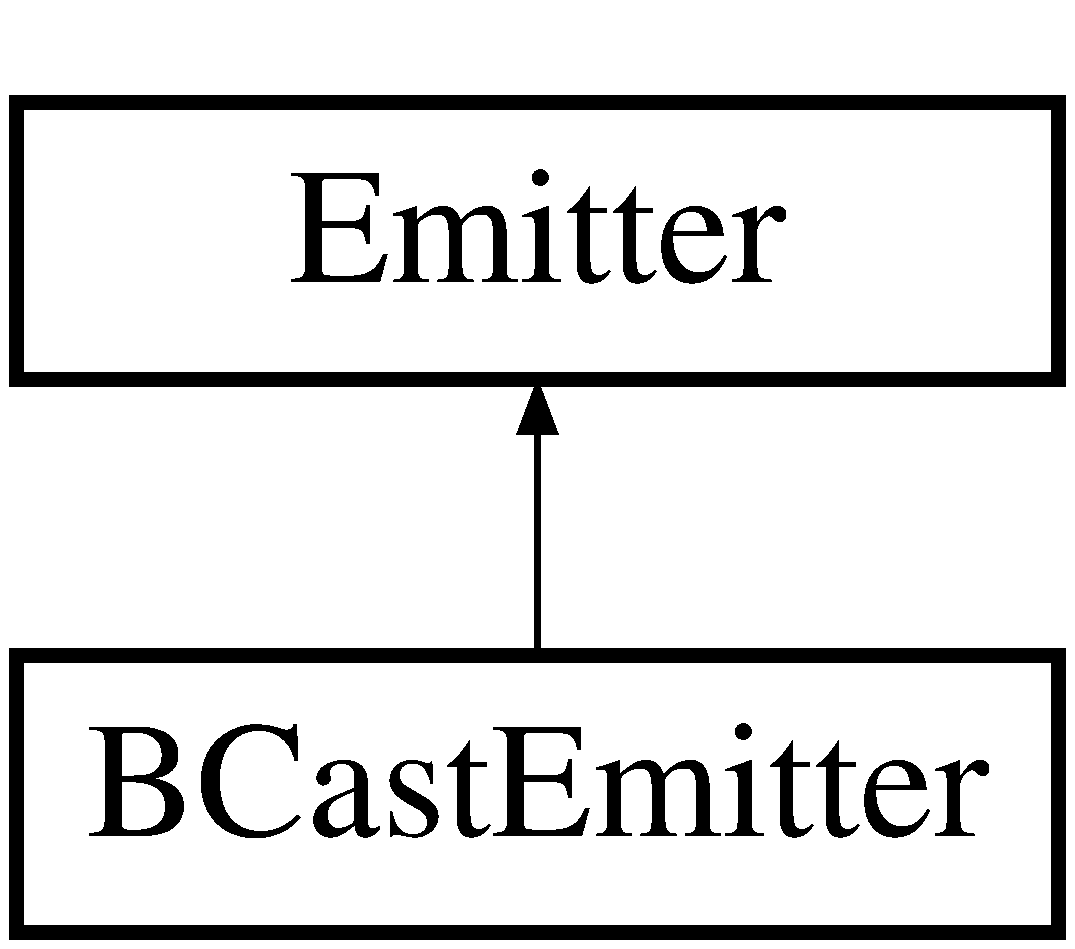
\includegraphics[height=2.000000cm]{class_b_cast_emitter}
\end{center}
\end{figure}
\subsection*{\-Public \-Member \-Functions}
\begin{DoxyCompactItemize}
\item 
\hypertarget{class_b_cast_emitter_a5d3a78dd06434eebf4ba82b00c1f358e}{{\bfseries \-B\-Cast\-Emitter} (size\-\_\-t nworkers\-\_\-, ff\-\_\-loadbalancer $\ast$const lb\-\_\-)}\label{class_b_cast_emitter_a5d3a78dd06434eebf4ba82b00c1f358e}

\item 
\hypertarget{class_b_cast_emitter_a48f1046a055b0d46ad9ebf551030dd23}{int {\bfseries svc\-\_\-init} ()}\label{class_b_cast_emitter_a48f1046a055b0d46ad9ebf551030dd23}

\item 
\hypertarget{class_b_cast_emitter_a771ab4e6eade9c5fa5c304b8c03256c3}{void $\ast$ {\bfseries svc} (void $\ast$task)}\label{class_b_cast_emitter_a771ab4e6eade9c5fa5c304b8c03256c3}

\end{DoxyCompactItemize}


\-The documentation for this class was generated from the following file\-:\begin{DoxyCompactItemize}
\item 
/home/travis/build/alpha-\/unito/\-Pi\-Co/\-Internals/\-F\-F\-Operators/\-B\-Cast\-Emitter.\-hpp\end{DoxyCompactItemize}

\hypertarget{class_binary_map}{\section{\-Binary\-Map$<$ \-In1, \-In2, \-Out $>$ \-Class \-Template \-Reference}
\label{class_binary_map}\index{\-Binary\-Map$<$ In1, In2, Out $>$@{\-Binary\-Map$<$ In1, In2, Out $>$}}
}


{\ttfamily \#include $<$\-Binary\-Map.\-hpp$>$}

\-Inheritance diagram for \-Binary\-Map$<$ \-In1, \-In2, \-Out $>$\-:\begin{figure}[H]
\begin{center}
\leavevmode
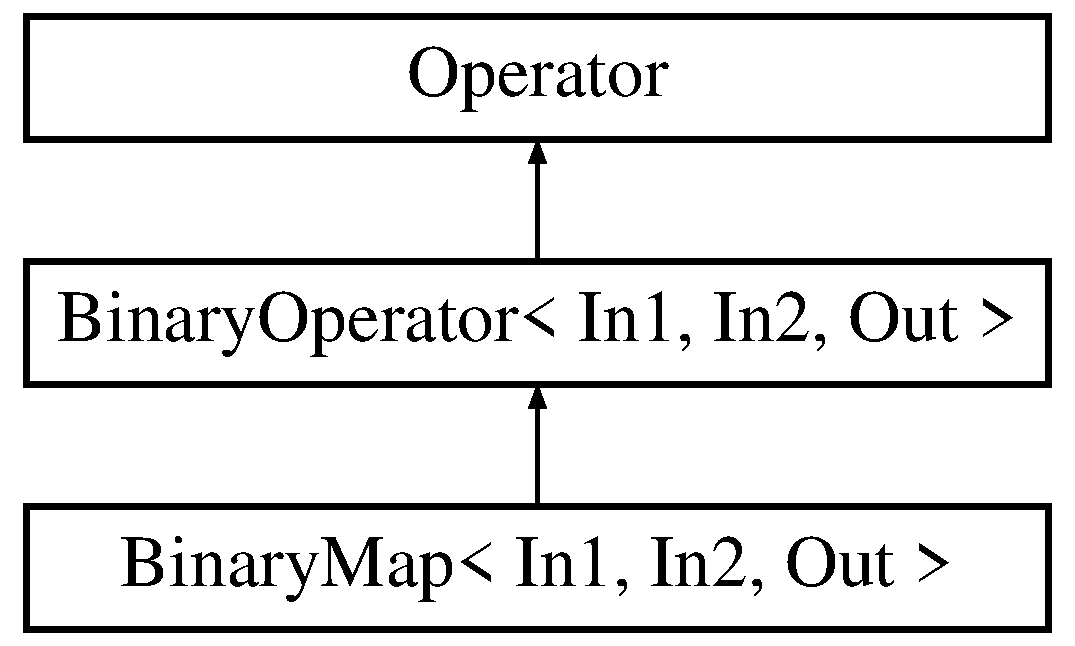
\includegraphics[height=3.000000cm]{class_binary_map}
\end{center}
\end{figure}
\subsection*{\-Public \-Member \-Functions}
\begin{DoxyCompactItemize}
\item 
\hyperlink{class_binary_map_abd8e19230ff0077f3782734313dafffc}{\-Binary\-Map} (std\-::function$<$ \-Out(\-In1, \-In2)$>$ bmapf\-\_\-)
\item 
std\-::string \hyperlink{class_binary_map_a891da29ca1c109f273e6b0448f261783}{name} ()
\item 
std\-::string \hyperlink{class_binary_map_a27f390ff0c80cdd9bc7b6361ed5df8c2}{name\-\_\-short} ()
\end{DoxyCompactItemize}
\subsection*{\-Protected \-Member \-Functions}
\begin{DoxyCompactItemize}
\item 
\hypertarget{class_binary_map_a4cb82813b17f67bc603e588b8590c315}{void {\bfseries run} ()}\label{class_binary_map_a4cb82813b17f67bc603e588b8590c315}

\item 
\hyperlink{class_binary_map}{\-Binary\-Map}$<$ \-In1, \-In2, \-Out $>$ $\ast$ \hyperlink{class_binary_map_a5ee518543d1593d6ae4a443b95461f70}{clone} ()
\item 
\hypertarget{class_binary_map_ab57a24e23e0a80e17f6b6a8bf2461d0e}{size\-\_\-t {\bfseries i\-\_\-degree} ()}\label{class_binary_map_ab57a24e23e0a80e17f6b6a8bf2461d0e}

\item 
\hypertarget{class_binary_map_a797b1d9ba0e907ed25865315e7e0dc1a}{size\-\_\-t {\bfseries o\-\_\-degree} ()}\label{class_binary_map_a797b1d9ba0e907ed25865315e7e0dc1a}

\item 
\hypertarget{class_binary_map_a2c00076ce44f296a9fc41994c2e3e162}{bool {\bfseries structure\-\_\-type} ()}\label{class_binary_map_a2c00076ce44f296a9fc41994c2e3e162}

\item 
\hypertarget{class_binary_map_a41145194d0d78b9eb3ad0b35ebd30da2}{const \-Operator\-Class {\bfseries operator\-\_\-class} ()}\label{class_binary_map_a41145194d0d78b9eb3ad0b35ebd30da2}

\item 
\hypertarget{class_binary_map_a25c286d36f6145f22ea5cf171b07103e}{ff\-::ff\-\_\-node $\ast$ {\bfseries node\-\_\-operator} (size\-\_\-t parallelism=1)}\label{class_binary_map_a25c286d36f6145f22ea5cf171b07103e}

\end{DoxyCompactItemize}
\subsection*{\-Friends}
\begin{DoxyCompactItemize}
\item 
\hypertarget{class_binary_map_adb788d0aa2d64624d3602a985936d7da}{class {\bfseries \-Pipe}}\label{class_binary_map_adb788d0aa2d64624d3602a985936d7da}

\end{DoxyCompactItemize}


\subsection{\-Detailed \-Description}
\subsubsection*{template$<$typename In1, typename In2, typename Out$>$class Binary\-Map$<$ In1, In2, Out $>$}

\-Defines an operator performing a binary \hyperlink{class_map}{\-Map}, taking in input two elements from two different input sources and producing a single output.

\-The \hyperlink{class_binary_map}{\-Binary\-Map} kernel is defined by the user and can be a lambda function, a functor or a function.

\-It implements a data-\/parallel operator that ignores any kind of grouping or windowing.

\-The kernel is applied independently to all the elements of both collections (either bounded or unbounded). 

\subsection{\-Constructor \& \-Destructor \-Documentation}
\hypertarget{class_binary_map_abd8e19230ff0077f3782734313dafffc}{\index{\-Binary\-Map@{\-Binary\-Map}!\-Binary\-Map@{\-Binary\-Map}}
\index{\-Binary\-Map@{\-Binary\-Map}!BinaryMap@{\-Binary\-Map}}
\subsubsection[{\-Binary\-Map}]{\setlength{\rightskip}{0pt plus 5cm}template$<$typename In1 , typename In2 , typename Out $>$ {\bf \-Binary\-Map}$<$ \-In1, \-In2, \-Out $>$\-::{\bf \-Binary\-Map} (
\begin{DoxyParamCaption}
\item[{std\-::function$<$ \-Out(\-In1, \-In2)$>$}]{bmapf\-\_\-}
\end{DoxyParamCaption}
)\hspace{0.3cm}{\ttfamily  \mbox{[}inline\mbox{]}}}}\label{class_binary_map_abd8e19230ff0077f3782734313dafffc}
\-Constructor. \-Creates a new \hyperlink{class_binary_map}{\-Binary\-Map} operator by defining its kernel function bmapf\-: $<$\-In1, \-In2$>$-\/$>$\-Out 
\begin{DoxyParams}{\-Parameters}
{\em bmapf} & std\-::function$<$\-Out(\-In1, In2)$>$ \hyperlink{class_binary_map}{\-Binary\-Map} kernel function with input types \-In1, \-In2 and producing an element of type \-Out \\
\hline
\end{DoxyParams}


\subsection{\-Member \-Function \-Documentation}
\hypertarget{class_binary_map_a5ee518543d1593d6ae4a443b95461f70}{\index{\-Binary\-Map@{\-Binary\-Map}!clone@{clone}}
\index{clone@{clone}!BinaryMap@{\-Binary\-Map}}
\subsubsection[{clone}]{\setlength{\rightskip}{0pt plus 5cm}template$<$typename In1 , typename In2 , typename Out $>$ {\bf \-Binary\-Map}$<$\-In1, \-In2, \-Out$>$$\ast$ {\bf \-Binary\-Map}$<$ \-In1, \-In2, \-Out $>$\-::{\bf clone} (
\begin{DoxyParamCaption}
{}
\end{DoxyParamCaption}
)\hspace{0.3cm}{\ttfamily  \mbox{[}inline, protected\mbox{]}}}}\label{class_binary_map_a5ee518543d1593d6ae4a443b95461f70}
\-Duplicates a \hyperlink{class_binary_map}{\-Binary\-Map} operator with a copy of the map kernel function. \begin{DoxyReturn}{\-Returns}
new \hyperlink{class_binary_map}{\-Binary\-Map} pointer 
\end{DoxyReturn}
\hypertarget{class_binary_map_a891da29ca1c109f273e6b0448f261783}{\index{\-Binary\-Map@{\-Binary\-Map}!name@{name}}
\index{name@{name}!BinaryMap@{\-Binary\-Map}}
\subsubsection[{name}]{\setlength{\rightskip}{0pt plus 5cm}template$<$typename In1 , typename In2 , typename Out $>$ std\-::string {\bf \-Binary\-Map}$<$ \-In1, \-In2, \-Out $>$\-::{\bf name} (
\begin{DoxyParamCaption}
{}
\end{DoxyParamCaption}
)\hspace{0.3cm}{\ttfamily  \mbox{[}inline, virtual\mbox{]}}}}\label{class_binary_map_a891da29ca1c109f273e6b0448f261783}
\-Returns a unique name for the operator. 

\-Implements \hyperlink{class_binary_operator_a6df8c4e6dee857f27d870c30d4f65920}{\-Binary\-Operator$<$ In1, In2, Out $>$}.

\hypertarget{class_binary_map_a27f390ff0c80cdd9bc7b6361ed5df8c2}{\index{\-Binary\-Map@{\-Binary\-Map}!name\-\_\-short@{name\-\_\-short}}
\index{name\-\_\-short@{name\-\_\-short}!BinaryMap@{\-Binary\-Map}}
\subsubsection[{name\-\_\-short}]{\setlength{\rightskip}{0pt plus 5cm}template$<$typename In1 , typename In2 , typename Out $>$ std\-::string {\bf \-Binary\-Map}$<$ \-In1, \-In2, \-Out $>$\-::{\bf name\-\_\-short} (
\begin{DoxyParamCaption}
{}
\end{DoxyParamCaption}
)\hspace{0.3cm}{\ttfamily  \mbox{[}inline, virtual\mbox{]}}}}\label{class_binary_map_a27f390ff0c80cdd9bc7b6361ed5df8c2}
\-Returns the name of the operator, consisting in the name of the class. 

\-Implements \hyperlink{class_operator}{\-Operator}.



\-The documentation for this class was generated from the following file\-:\begin{DoxyCompactItemize}
\item 
/home/travis/build/alpha-\/unito/\-Pi\-Co/\-Operators/\-Binary\-Map.\-hpp\end{DoxyCompactItemize}

\hypertarget{class_binary_operator}{\section{\-Binary\-Operator$<$ \-In1, \-In2, \-Out $>$ \-Class \-Template \-Reference}
\label{class_binary_operator}\index{\-Binary\-Operator$<$ In1, In2, Out $>$@{\-Binary\-Operator$<$ In1, In2, Out $>$}}
}


{\ttfamily \#include $<$\-Binary\-Operator.\-hpp$>$}

\-Inheritance diagram for \-Binary\-Operator$<$ \-In1, \-In2, \-Out $>$\-:\begin{figure}[H]
\begin{center}
\leavevmode
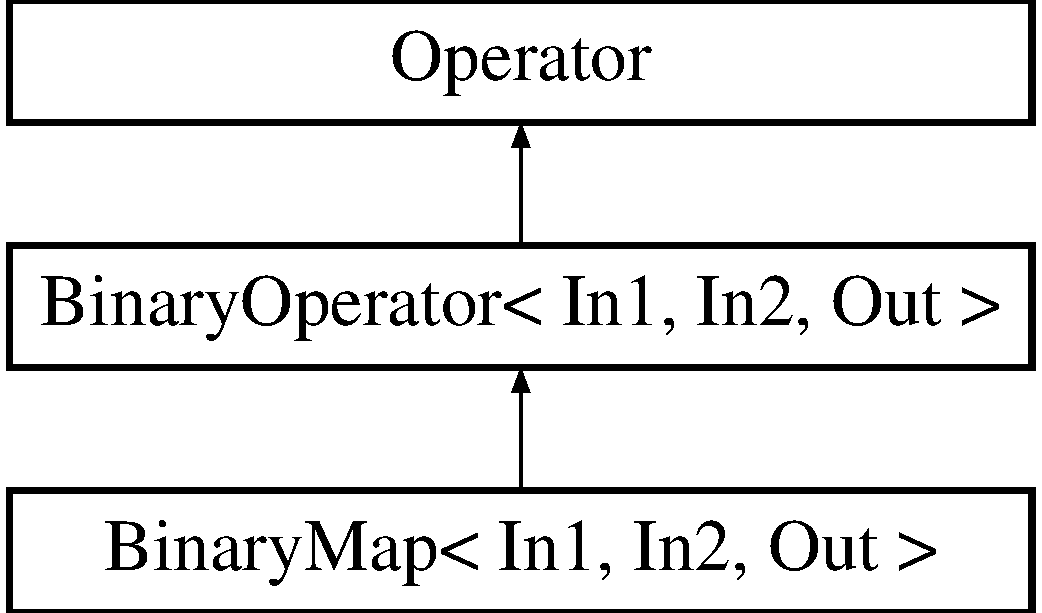
\includegraphics[height=3.000000cm]{class_binary_operator}
\end{center}
\end{figure}
\subsection*{\-Public \-Member \-Functions}
\begin{DoxyCompactItemize}
\item 
virtual std\-::string \hyperlink{class_binary_operator_a6df8c4e6dee857f27d870c30d4f65920}{name} ()=0
\end{DoxyCompactItemize}
\subsection*{\-Protected \-Member \-Functions}
\begin{DoxyCompactItemize}
\item 
\hypertarget{class_binary_operator_a2de8a96fc037a231f39b3118069f5b08}{virtual bool {\bfseries check\-Input\-Type\-Sanity} (\-Type\-Info\-Ref id)}\label{class_binary_operator_a2de8a96fc037a231f39b3118069f5b08}

\item 
\hypertarget{class_binary_operator_a90a60672775f8d7958dda0600c5ed546}{virtual bool {\bfseries check\-Output\-Type\-Sanity} (\-Type\-Info\-Ref id)}\label{class_binary_operator_a90a60672775f8d7958dda0600c5ed546}

\item 
\hypertarget{class_binary_operator_a97a69de42fae8bab00c814459ea844b0}{virtual size\-\_\-t {\bfseries i\-\_\-degree} ()=0}\label{class_binary_operator_a97a69de42fae8bab00c814459ea844b0}

\item 
\hypertarget{class_binary_operator_aee9650145b55dfcd040042d9be249171}{virtual size\-\_\-t {\bfseries o\-\_\-degree} ()=0}\label{class_binary_operator_aee9650145b55dfcd040042d9be249171}

\item 
\hypertarget{class_binary_operator_a2fc538f30e110d6313bad1066236143b}{virtual bool $\ast$ {\bfseries structure\-\_\-type} ()=0}\label{class_binary_operator_a2fc538f30e110d6313bad1066236143b}

\item 
\hypertarget{class_binary_operator_a8c247face4b17579873d45b4b14df527}{virtual const \-Operator\-Class {\bfseries operator\-\_\-class} ()=0}\label{class_binary_operator_a8c247face4b17579873d45b4b14df527}

\item 
\hypertarget{class_binary_operator_aeedefcb624a8ab84b10bbab872df72e4}{virtual ff\-::ff\-\_\-node $\ast$ {\bfseries node\-\_\-operator} (size\-\_\-t parallelism=1)=0}\label{class_binary_operator_aeedefcb624a8ab84b10bbab872df72e4}

\end{DoxyCompactItemize}
\subsection*{\-Friends}
\begin{DoxyCompactItemize}
\item 
\hypertarget{class_binary_operator_adb788d0aa2d64624d3602a985936d7da}{class {\bfseries \-Pipe}}\label{class_binary_operator_adb788d0aa2d64624d3602a985936d7da}

\end{DoxyCompactItemize}


\subsection{\-Detailed \-Description}
\subsubsection*{template$<$typename \-In1, typename \-In2, typename \-Out$>$class Binary\-Operator$<$ In1, In2, Out $>$}

\-Base class for actor nodes with $\ast$two$\ast$ input streams and $\ast$one$\ast$ output stream, either bound or unbound and grouped or plain. \-It is provided with methods for input/output type checking. 

\subsection{\-Member \-Function \-Documentation}
\hypertarget{class_binary_operator_a6df8c4e6dee857f27d870c30d4f65920}{\index{\-Binary\-Operator@{\-Binary\-Operator}!name@{name}}
\index{name@{name}!BinaryOperator@{\-Binary\-Operator}}
\subsubsection[{name}]{\setlength{\rightskip}{0pt plus 5cm}template$<$typename \-In1, typename \-In2, typename \-Out$>$ virtual std\-::string {\bf \-Binary\-Operator}$<$ \-In1, \-In2, \-Out $>$\-::{\bf name} (
\begin{DoxyParamCaption}
{}
\end{DoxyParamCaption}
)\hspace{0.3cm}{\ttfamily  \mbox{[}pure virtual\mbox{]}}}}\label{class_binary_operator_a6df8c4e6dee857f27d870c30d4f65920}
\-Returns a unique name for the operator. 

\-Reimplemented from \hyperlink{class_operator_aabb42a0bffefa195ef28dcb8de28aec1}{\-Operator}.



\-Implemented in \hyperlink{class_binary_map_a891da29ca1c109f273e6b0448f261783}{\-Binary\-Map$<$ In1, In2, Out $>$}.



\-The documentation for this class was generated from the following file\-:\begin{DoxyCompactItemize}
\item 
/home/travis/build/alpha-\/unito/\-Pi\-Co/\-Operators/\-Binary\-Operator.\-hpp\end{DoxyCompactItemize}

\hypertarget{class_collector}{\section{\-Collector \-Class \-Reference}
\label{class_collector}\index{\-Collector@{\-Collector}}
}
\subsection*{\-Public \-Member \-Functions}
\begin{DoxyCompactItemize}
\item 
\hypertarget{class_collector_a73d4be8c9cfac5b54c0b376bb3951175}{int {\bfseries svc\-\_\-init} ()}\label{class_collector_a73d4be8c9cfac5b54c0b376bb3951175}

\item 
\hypertarget{class_collector_a26fd5886929719be749dd53a77039ca0}{void $\ast$ {\bfseries svc} (void $\ast$task)}\label{class_collector_a26fd5886929719be749dd53a77039ca0}

\end{DoxyCompactItemize}


\-The documentation for this class was generated from the following file\-:\begin{DoxyCompactItemize}
\item 
/home/travis/build/alpha-\/unito/\-Pi\-Co/\-Internals/\-F\-F\-Operators/\-Collector.\-hpp\end{DoxyCompactItemize}

\hypertarget{class_emitter}{\section{\-Emitter \-Class \-Reference}
\label{class_emitter}\index{\-Emitter@{\-Emitter}}
}
\-Inheritance diagram for \-Emitter\-:\begin{figure}[H]
\begin{center}
\leavevmode
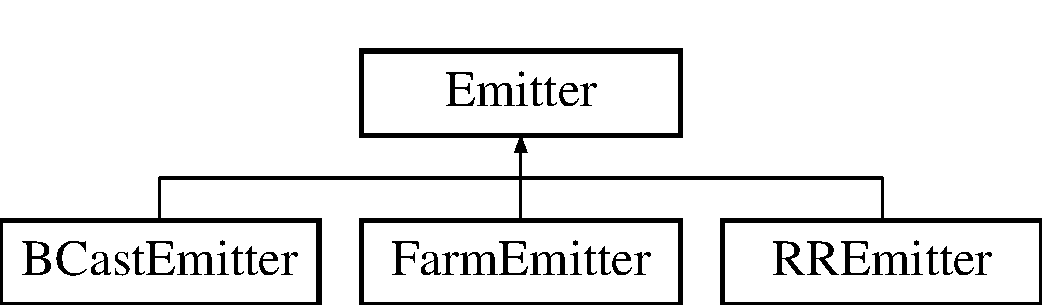
\includegraphics[height=2.000000cm]{class_emitter}
\end{center}
\end{figure}


\-The documentation for this class was generated from the following file\-:\begin{DoxyCompactItemize}
\item 
/home/travis/build/alpha-\/unito/\-Pi\-Co/\-Internals/\-F\-F\-Operators/\-Emitter.\-hpp\end{DoxyCompactItemize}

\hypertarget{class_flat_map}{\section{\-Flat\-Map$<$ \-In, \-Out $>$ \-Class \-Template \-Reference}
\label{class_flat_map}\index{\-Flat\-Map$<$ In, Out $>$@{\-Flat\-Map$<$ In, Out $>$}}
}


{\ttfamily \#include $<$\-Flat\-Map.\-hpp$>$}

\-Inheritance diagram for \-Flat\-Map$<$ \-In, \-Out $>$\-:\begin{figure}[H]
\begin{center}
\leavevmode
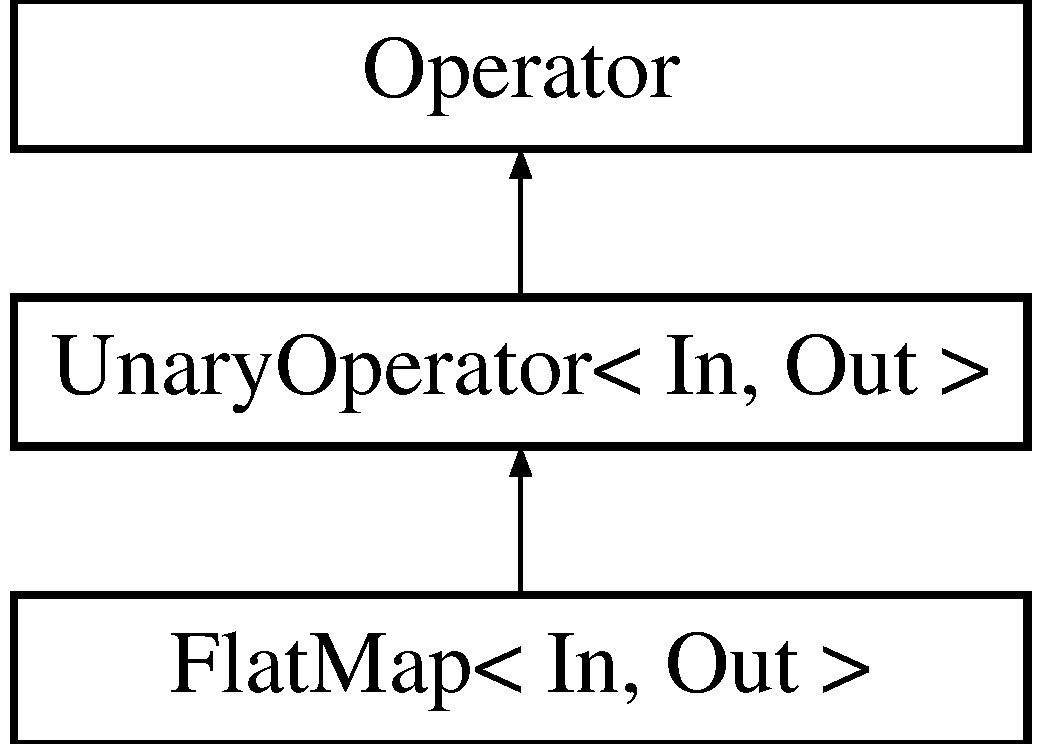
\includegraphics[height=3.000000cm]{class_flat_map}
\end{center}
\end{figure}
\subsection*{\-Public \-Member \-Functions}
\begin{DoxyCompactItemize}
\item 
\hyperlink{class_flat_map_a8ec8c425acf80cf2577b434b195904bd}{\-Flat\-Map} (std\-::function$<$ std\-::vector$<$ \-Out $>$(\-In)$>$ flatmapf\-\_\-)
\item 
std\-::string \hyperlink{class_flat_map_ae5ead8986dd0847b81a65c4857e856c7}{name\-\_\-short} ()
\end{DoxyCompactItemize}
\subsection*{\-Protected \-Member \-Functions}
\begin{DoxyCompactItemize}
\item 
\hypertarget{class_flat_map_ac02777613b25e9fcf563d3060a9fde26}{void {\bfseries run} (\-In $\ast$task)}\label{class_flat_map_ac02777613b25e9fcf563d3060a9fde26}

\item 
\hypertarget{class_flat_map_a448c6f98264a251bb8fb691c94bf2556}{const \-Operator\-Class {\bfseries operator\-\_\-class} ()}\label{class_flat_map_a448c6f98264a251bb8fb691c94bf2556}

\item 
\hypertarget{class_flat_map_abc46d83d6c841e3113f611ab5f9ab48f}{ff\-::ff\-\_\-node $\ast$ {\bfseries node\-\_\-operator} (size\-\_\-t par\-\_\-deg=1)}\label{class_flat_map_abc46d83d6c841e3113f611ab5f9ab48f}

\end{DoxyCompactItemize}
\subsection*{\-Friends}
\begin{DoxyCompactItemize}
\item 
\hypertarget{class_flat_map_adb788d0aa2d64624d3602a985936d7da}{class {\bfseries \-Pipe}}\label{class_flat_map_adb788d0aa2d64624d3602a985936d7da}

\end{DoxyCompactItemize}


\subsection{\-Detailed \-Description}
\subsubsection*{template$<$typename In, typename Out$>$class Flat\-Map$<$ In, Out $>$}

\-Defines an operator performing a \hyperlink{class_flat_map}{\-Flat\-Map}, taking in input one element from the input source and producing zero, one or more elements in output. \-The \hyperlink{class_flat_map}{\-Flat\-Map} kernel is defined by the user and can be a lambda function, a functor or a function.

\-It implements a data-\/parallel operator that ignores any kind of grouping or windowing.

\-The kernel is applied independently to all the elements of the collection (either bounded or unbounded). 

\subsection{\-Constructor \& \-Destructor \-Documentation}
\hypertarget{class_flat_map_a8ec8c425acf80cf2577b434b195904bd}{\index{\-Flat\-Map@{\-Flat\-Map}!\-Flat\-Map@{\-Flat\-Map}}
\index{\-Flat\-Map@{\-Flat\-Map}!FlatMap@{\-Flat\-Map}}
\subsubsection[{\-Flat\-Map}]{\setlength{\rightskip}{0pt plus 5cm}template$<$typename In , typename Out $>$ {\bf \-Flat\-Map}$<$ \-In, \-Out $>$\-::{\bf \-Flat\-Map} (
\begin{DoxyParamCaption}
\item[{std\-::function$<$ std\-::vector$<$ \-Out $>$(\-In)$>$}]{flatmapf\-\_\-}
\end{DoxyParamCaption}
)\hspace{0.3cm}{\ttfamily  \mbox{[}inline\mbox{]}}}}\label{class_flat_map_a8ec8c425acf80cf2577b434b195904bd}
\-Constructor. \-Creates a new \hyperlink{class_flat_map}{\-Flat\-Map} operator by defining its kernel function flat\-Mapf\-: \-In-\/$>$\-Out 
\begin{DoxyParams}{\-Parameters}
{\em flatmapf} & std\-::function$<$\-Out(\-In)$>$ \hyperlink{class_flat_map}{\-Flat\-Map} kernel function with input type \-In producing zero, one or more element of type \-Out \\
\hline
\end{DoxyParams}


\subsection{\-Member \-Function \-Documentation}
\hypertarget{class_flat_map_ae5ead8986dd0847b81a65c4857e856c7}{\index{\-Flat\-Map@{\-Flat\-Map}!name\-\_\-short@{name\-\_\-short}}
\index{name\-\_\-short@{name\-\_\-short}!FlatMap@{\-Flat\-Map}}
\subsubsection[{name\-\_\-short}]{\setlength{\rightskip}{0pt plus 5cm}template$<$typename In , typename Out $>$ std\-::string {\bf \-Flat\-Map}$<$ \-In, \-Out $>$\-::{\bf name\-\_\-short} (
\begin{DoxyParamCaption}
{}
\end{DoxyParamCaption}
)\hspace{0.3cm}{\ttfamily  \mbox{[}inline, virtual\mbox{]}}}}\label{class_flat_map_ae5ead8986dd0847b81a65c4857e856c7}
\-Returns the name of the operator, consisting in the name of the class. 

\-Implements \hyperlink{class_operator}{\-Operator}.



\-The documentation for this class was generated from the following file\-:\begin{DoxyCompactItemize}
\item 
/home/travis/build/alpha-\/unito/\-Pi\-Co/\-Operators/\-Flat\-Map.\-hpp\end{DoxyCompactItemize}

\hypertarget{class_group_param}{\section{\-Group\-Param \-Class \-Reference}
\label{class_group_param}\index{\-Group\-Param@{\-Group\-Param}}
}


\-The documentation for this class was generated from the following file\-:\begin{DoxyCompactItemize}
\item 
/home/travis/build/alpha-\/unito/\-Pi\-Co/\-Internals/\-Group\-Param.\-hpp\end{DoxyCompactItemize}

\hypertarget{class_input_operator}{\section{\-Input\-Operator$<$ \-Out $>$ \-Class \-Template \-Reference}
\label{class_input_operator}\index{\-Input\-Operator$<$ Out $>$@{\-Input\-Operator$<$ Out $>$}}
}


{\ttfamily \#include $<$\-Input\-Operator.\-hpp$>$}

\-Inheritance diagram for \-Input\-Operator$<$ \-Out $>$\-:\begin{figure}[H]
\begin{center}
\leavevmode
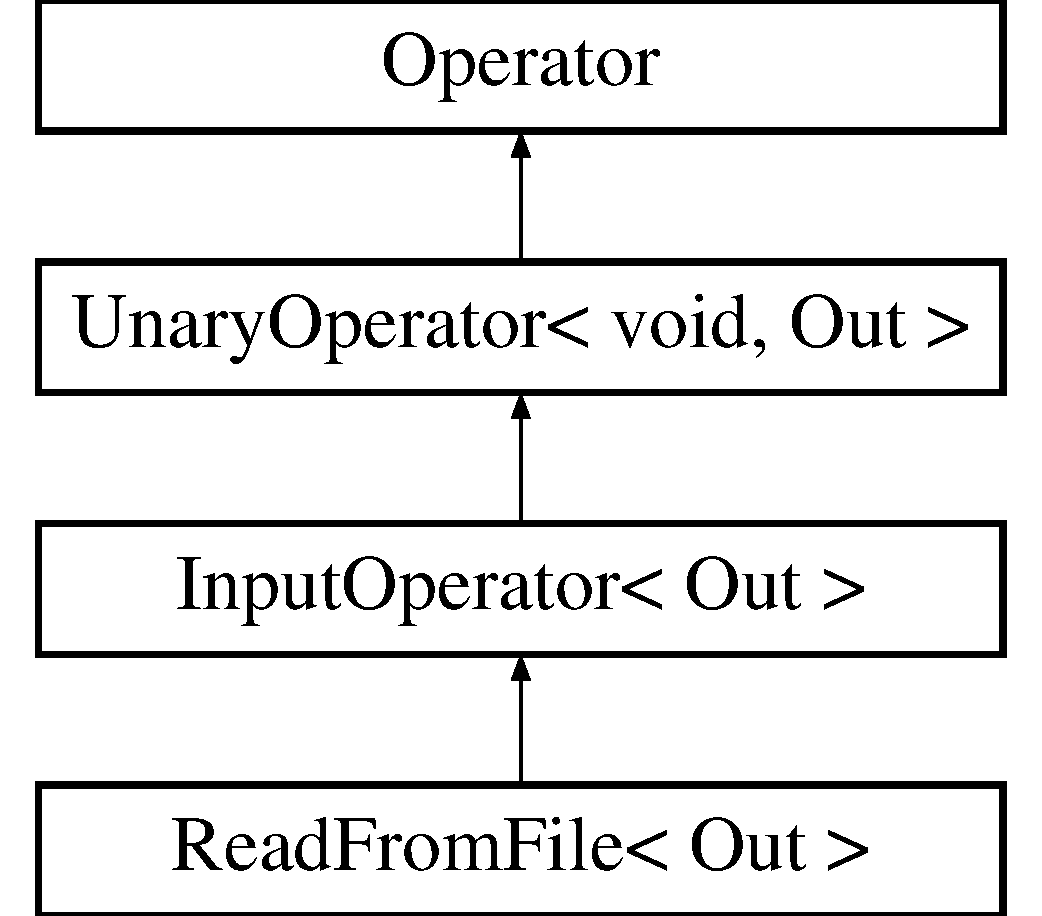
\includegraphics[height=4.000000cm]{class_input_operator}
\end{center}
\end{figure}
\subsection*{\-Public \-Member \-Functions}
\begin{DoxyCompactItemize}
\item 
\hyperlink{class_input_operator_a70a9e8ae6fc3e6bee0b7f1e422f7cee6}{\-Input\-Operator} (\-Structure\-Type st\-\_\-)
\item 
\hyperlink{class_input_operator_a76e4803ef97f634399cb9de1d5ec1be7}{\-Input\-Operator} (const \hyperlink{class_input_operator}{\-Input\-Operator} \&copy)
\item 
std\-::string \hyperlink{class_input_operator_a5f752278e586f9c22535bdffdbbe14d2}{name\-\_\-short} ()
\item 
\hypertarget{class_input_operator_ab0266126058393d30ffa92b7cf408d32}{virtual void {\bfseries run\-\_\-kernel} ()=0}\label{class_input_operator_ab0266126058393d30ffa92b7cf408d32}

\end{DoxyCompactItemize}
\subsection*{\-Protected \-Member \-Functions}
\begin{DoxyCompactItemize}
\item 
\hypertarget{class_input_operator_a370bbb3a5c72e0121448e8c06ae1fe28}{const \-Operator\-Class {\bfseries operator\-\_\-class} ()}\label{class_input_operator_a370bbb3a5c72e0121448e8c06ae1fe28}

\end{DoxyCompactItemize}


\subsection{\-Detailed \-Description}
\subsubsection*{template$<$typename Out$>$class Input\-Operator$<$ Out $>$}

\-Defines an operator performing the policy for generating input (i.\-e. read from file).

\-The input generation kernel is defined by the user and can be a lambda function, a functor or a function.

\-Furthermore, the user specifies the structure of the data type the \hyperlink{class_emitter}{\-Emitter} generates. \-It can be\-:
\begin{DoxyItemize}
\item \-Bag (spec\-: unordered, bounded)
\item \-List (spec\-: ordered, bounded)
\item \-Stream (spec\-: ordered, unbounded)
\item \-Unbounded \-Bag (spec\-: unordered, unbounded)
\end{DoxyItemize}

\-The operator is global and unique for the \hyperlink{class_pipe}{\-Pipe} it refers to. 

\subsection{\-Constructor \& \-Destructor \-Documentation}
\hypertarget{class_input_operator_a70a9e8ae6fc3e6bee0b7f1e422f7cee6}{\index{\-Input\-Operator@{\-Input\-Operator}!\-Input\-Operator@{\-Input\-Operator}}
\index{\-Input\-Operator@{\-Input\-Operator}!InputOperator@{\-Input\-Operator}}
\subsubsection[{\-Input\-Operator}]{\setlength{\rightskip}{0pt plus 5cm}template$<$typename Out $>$ {\bf \-Input\-Operator}$<$ \-Out $>$\-::{\bf \-Input\-Operator} (
\begin{DoxyParamCaption}
\item[{\-Structure\-Type}]{st\-\_\-}
\end{DoxyParamCaption}
)\hspace{0.3cm}{\ttfamily  \mbox{[}inline\mbox{]}}}}\label{class_input_operator_a70a9e8ae6fc3e6bee0b7f1e422f7cee6}
\-Constructor. \-Creates a new \hyperlink{class_emitter}{\-Emitter} by defining its kernel function genf\-: void -\/$>$ \-Out operating on a specified datatype. \hypertarget{class_input_operator_a76e4803ef97f634399cb9de1d5ec1be7}{\index{\-Input\-Operator@{\-Input\-Operator}!\-Input\-Operator@{\-Input\-Operator}}
\index{\-Input\-Operator@{\-Input\-Operator}!InputOperator@{\-Input\-Operator}}
\subsubsection[{\-Input\-Operator}]{\setlength{\rightskip}{0pt plus 5cm}template$<$typename Out $>$ {\bf \-Input\-Operator}$<$ \-Out $>$\-::{\bf \-Input\-Operator} (
\begin{DoxyParamCaption}
\item[{const {\bf \-Input\-Operator}$<$ \-Out $>$ \&}]{copy}
\end{DoxyParamCaption}
)\hspace{0.3cm}{\ttfamily  \mbox{[}inline\mbox{]}}}}\label{class_input_operator_a76e4803ef97f634399cb9de1d5ec1be7}
\-Copy constructor 

\subsection{\-Member \-Function \-Documentation}
\hypertarget{class_input_operator_a5f752278e586f9c22535bdffdbbe14d2}{\index{\-Input\-Operator@{\-Input\-Operator}!name\-\_\-short@{name\-\_\-short}}
\index{name\-\_\-short@{name\-\_\-short}!InputOperator@{\-Input\-Operator}}
\subsubsection[{name\-\_\-short}]{\setlength{\rightskip}{0pt plus 5cm}template$<$typename Out $>$ std\-::string {\bf \-Input\-Operator}$<$ \-Out $>$\-::{\bf name\-\_\-short} (
\begin{DoxyParamCaption}
{}
\end{DoxyParamCaption}
)\hspace{0.3cm}{\ttfamily  \mbox{[}inline, virtual\mbox{]}}}}\label{class_input_operator_a5f752278e586f9c22535bdffdbbe14d2}
\-Returns the name of the operator, consisting in the name of the class. 

\-Implements \hyperlink{class_operator}{\-Operator}.



\-Reimplemented in \hyperlink{class_read_from_file_a58ff16dcafb4ad2039cf151fd7a0440f}{\-Read\-From\-File$<$ Out $>$}.



\-The documentation for this class was generated from the following file\-:\begin{DoxyCompactItemize}
\item 
/home/travis/build/alpha-\/unito/\-Pi\-Co/\-Operators/\-In\-Out/\-Input\-Operator.\-hpp\end{DoxyCompactItemize}

\hypertarget{class_key_value}{\section{\-Key\-Value$<$ \-K, \-V $>$ \-Class \-Template \-Reference}
\label{class_key_value}\index{\-Key\-Value$<$ K, V $>$@{\-Key\-Value$<$ K, V $>$}}
}
\subsection*{\-Public \-Types}
\begin{DoxyCompactItemize}
\item 
\hypertarget{class_key_value_ae1cb822a5b7f44313b8b15b05297793c}{typedef \-K {\bfseries keytype}}\label{class_key_value_ae1cb822a5b7f44313b8b15b05297793c}

\end{DoxyCompactItemize}
\subsection*{\-Public \-Member \-Functions}
\begin{DoxyCompactItemize}
\item 
\hypertarget{class_key_value_a7db11022344a7b927223f3e87fa63e69}{{\bfseries \-Key\-Value} (\-K key\-\_\-, \-V val\-\_\-)}\label{class_key_value_a7db11022344a7b927223f3e87fa63e69}

\item 
\hypertarget{class_key_value_ae4ea8e7bf68b0bae160108622497c287}{{\bfseries \-Key\-Value} (const \hyperlink{class_key_value}{\-Key\-Value} \&kv)}\label{class_key_value_ae4ea8e7bf68b0bae160108622497c287}

\item 
\hypertarget{class_key_value_a39f6e53de9df547cd6b9f6e414f95f01}{const \-K \& {\bfseries \-Key} () const }\label{class_key_value_a39f6e53de9df547cd6b9f6e414f95f01}

\item 
\hypertarget{class_key_value_a24db94572b5cb3117524f91f7927d8b8}{const \-V \& {\bfseries \-Value} () const }\label{class_key_value_a24db94572b5cb3117524f91f7927d8b8}

\item 
\hypertarget{class_key_value_a6ae6fdd42f97db278f44b1fd247f5e26}{void {\bfseries \-Key} (\-K key\-\_\-)}\label{class_key_value_a6ae6fdd42f97db278f44b1fd247f5e26}

\item 
\hypertarget{class_key_value_ada87254eda6cc833578d5a001c3c08e7}{void {\bfseries \-Value} (\-V val\-\_\-)}\label{class_key_value_ada87254eda6cc833578d5a001c3c08e7}

\item 
\hypertarget{class_key_value_ae093f9a98b1d9670f386e2f008f5a97b}{void {\bfseries \-Key\-Val} (\-K key\-\_\-, \-V val\-\_\-)}\label{class_key_value_ae093f9a98b1d9670f386e2f008f5a97b}

\item 
\hypertarget{class_key_value_ad9fc3e92e9ccc30350da0ad4e5e7100e}{void {\bfseries operator=} (const \hyperlink{class_key_value}{\-Key\-Value} \&kv)}\label{class_key_value_ad9fc3e92e9ccc30350da0ad4e5e7100e}

\item 
\hypertarget{class_key_value_abb0770976789c796d9e1f2cc12968bea}{bool {\bfseries operator==} (\hyperlink{class_key_value}{\-Key\-Value} \&kv)}\label{class_key_value_abb0770976789c796d9e1f2cc12968bea}

\item 
\hypertarget{class_key_value_a1996c53df43ccb7b5b9ce5ca2ab86a24}{void {\bfseries sum\-Value} (const \hyperlink{class_key_value}{\-Key\-Value} \&kv)}\label{class_key_value_a1996c53df43ccb7b5b9ce5ca2ab86a24}

\item 
\hypertarget{class_key_value_a64e6a339b308fb94e3d62f10d2ac2478}{bool {\bfseries same\-Key} (const \hyperlink{class_key_value}{\-Key\-Value} \&kv) const }\label{class_key_value_a64e6a339b308fb94e3d62f10d2ac2478}

\end{DoxyCompactItemize}
\subsection*{\-Friends}
\begin{DoxyCompactItemize}
\item 
\hypertarget{class_key_value_a39c082a850561b5283e7bf5858a88cac}{std\-::ostream \& {\bfseries operator$<$$<$} (std\-::ostream \&os, const \hyperlink{class_key_value}{\-Key\-Value} \&kv)}\label{class_key_value_a39c082a850561b5283e7bf5858a88cac}

\item 
\hypertarget{class_key_value_a60405bd4e3c6371f045b28bb6100c58b}{\hyperlink{class_key_value}{\-Key\-Value} {\bfseries operator+} (\hyperlink{class_key_value}{\-Key\-Value} lhs, const \hyperlink{class_key_value}{\-Key\-Value} \&rhs)}\label{class_key_value_a60405bd4e3c6371f045b28bb6100c58b}

\end{DoxyCompactItemize}
\subsubsection*{template$<$typename K, typename V$>$ class Key\-Value$<$ K, V $>$}



\-The documentation for this class was generated from the following file\-:\begin{DoxyCompactItemize}
\item 
/home/travis/build/alpha-\/unito/\-Pi\-Co/\-Internals/\-Types/\-Key\-Value.\-hpp\end{DoxyCompactItemize}

\hypertarget{class_map}{\section{\-Map$<$ \-In, \-Out $>$ \-Class \-Template \-Reference}
\label{class_map}\index{\-Map$<$ In, Out $>$@{\-Map$<$ In, Out $>$}}
}


{\ttfamily \#include $<$\-Map.\-hpp$>$}

\-Inheritance diagram for \-Map$<$ \-In, \-Out $>$\-:\begin{figure}[H]
\begin{center}
\leavevmode
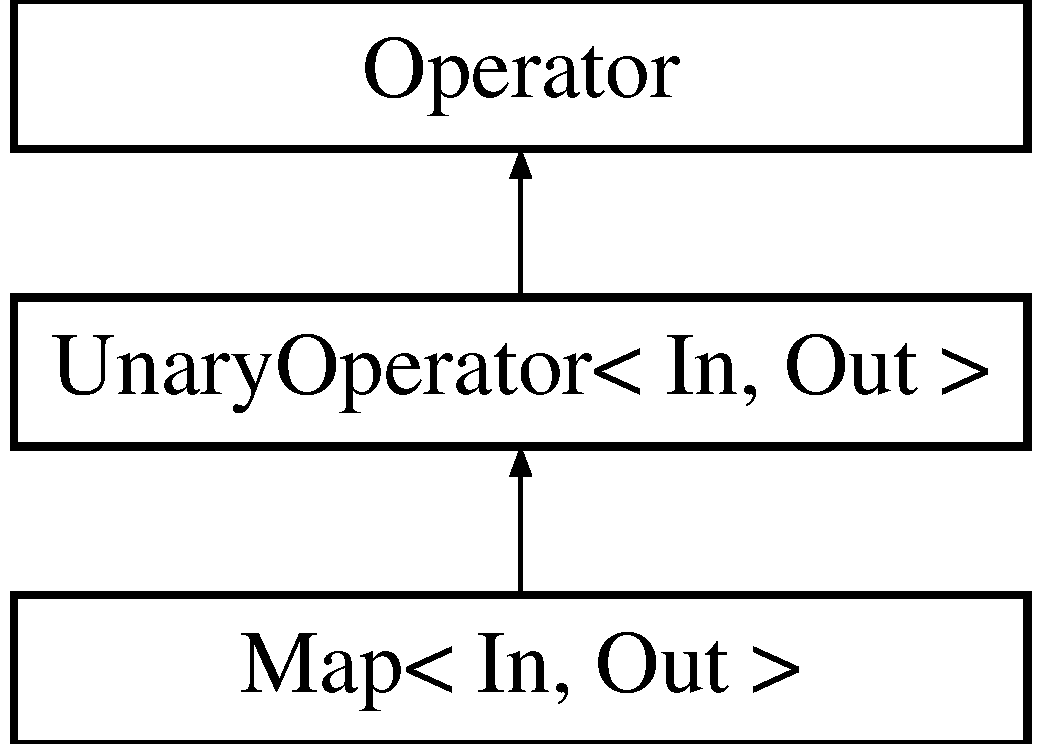
\includegraphics[height=3.000000cm]{class_map}
\end{center}
\end{figure}
\subsection*{\-Public \-Member \-Functions}
\begin{DoxyCompactItemize}
\item 
\hyperlink{class_map_a592d69e973dc2596ab688914fb7f5f65}{\-Map} (std\-::function$<$ \-Out(\-In)$>$ mapf\-\_\-)
\item 
std\-::string \hyperlink{class_map_a0ac45a1807983af02472c0a01994bf61}{name\-\_\-short} ()
\end{DoxyCompactItemize}
\subsection*{\-Protected \-Member \-Functions}
\begin{DoxyCompactItemize}
\item 
\hypertarget{class_map_ae61a30423820caac53954f22c5935580}{\-Out {\bfseries run\-\_\-kernel} (\-In $\ast$in\-\_\-task)}\label{class_map_ae61a30423820caac53954f22c5935580}

\item 
\hyperlink{class_map}{\-Map}$<$ \-In, \-Out $>$ $\ast$ \hyperlink{class_map_a0524200b07c1713bc9f3dd60b372b30c}{clone} ()
\item 
\hypertarget{class_map_a5c9fcf56ffe1fd40d3642bcfc561844a}{const \-Operator\-Class {\bfseries operator\-\_\-class} ()}\label{class_map_a5c9fcf56ffe1fd40d3642bcfc561844a}

\item 
\hypertarget{class_map_ae0cc5feac0abb9c2a7cad61dbf50157e}{ff\-::ff\-\_\-node $\ast$ {\bfseries node\-\_\-operator} (size\-\_\-t parallelism=1)}\label{class_map_ae0cc5feac0abb9c2a7cad61dbf50157e}

\end{DoxyCompactItemize}
\subsection*{\-Friends}
\begin{DoxyCompactItemize}
\item 
\hypertarget{class_map_adb788d0aa2d64624d3602a985936d7da}{class {\bfseries \-Pipe}}\label{class_map_adb788d0aa2d64624d3602a985936d7da}

\item 
\hypertarget{class_map_a298bf270ce895db324d65478b3b01f5b}{class {\bfseries \-Par\-Exec\-D\-F}}\label{class_map_a298bf270ce895db324d65478b3b01f5b}

\end{DoxyCompactItemize}


\subsection{\-Detailed \-Description}
\subsubsection*{template$<$typename In, typename Out$>$class Map$<$ In, Out $>$}

\-Defines an operator performing a \hyperlink{class_map}{\-Map} function, taking in input one element from the input source and producing one in output. \-The \hyperlink{class_map}{\-Map} kernel is defined by the user and can be a lambda function, a functor or a function.

\-It implements a data-\/parallel operator that ignores any kind of grouping or windowing.

\-The kernel is applied independently to all the elements of the collection (either bounded or unbounded). 

\subsection{\-Constructor \& \-Destructor \-Documentation}
\hypertarget{class_map_a592d69e973dc2596ab688914fb7f5f65}{\index{\-Map@{\-Map}!\-Map@{\-Map}}
\index{\-Map@{\-Map}!Map@{\-Map}}
\subsubsection[{\-Map}]{\setlength{\rightskip}{0pt plus 5cm}template$<$typename In , typename Out $>$ {\bf \-Map}$<$ \-In, \-Out $>$\-::{\bf \-Map} (
\begin{DoxyParamCaption}
\item[{std\-::function$<$ \-Out(\-In)$>$}]{mapf\-\_\-}
\end{DoxyParamCaption}
)\hspace{0.3cm}{\ttfamily  \mbox{[}inline\mbox{]}}}}\label{class_map_a592d69e973dc2596ab688914fb7f5f65}
\-Constructor. \-Creates a new \hyperlink{class_map}{\-Map} operator by defining its kernel function mapf\-: \-In-\/$>$\-Out 
\begin{DoxyParams}{\-Parameters}
{\em mapf} & std\-::function$<$\-Out(\-In)$>$ \hyperlink{class_map}{\-Map} kernel function with input type \-In producing an element of type \-Out \\
\hline
\end{DoxyParams}


\subsection{\-Member \-Function \-Documentation}
\hypertarget{class_map_a0524200b07c1713bc9f3dd60b372b30c}{\index{\-Map@{\-Map}!clone@{clone}}
\index{clone@{clone}!Map@{\-Map}}
\subsubsection[{clone}]{\setlength{\rightskip}{0pt plus 5cm}template$<$typename In , typename Out $>$ {\bf \-Map}$<$\-In, \-Out$>$$\ast$ {\bf \-Map}$<$ \-In, \-Out $>$\-::{\bf clone} (
\begin{DoxyParamCaption}
{}
\end{DoxyParamCaption}
)\hspace{0.3cm}{\ttfamily  \mbox{[}inline, protected\mbox{]}}}}\label{class_map_a0524200b07c1713bc9f3dd60b372b30c}
\-Duplicates a \hyperlink{class_map}{\-Map} with a copy of the \hyperlink{class_map}{\-Map} kernel function. \begin{DoxyReturn}{\-Returns}
new \hyperlink{class_map}{\-Map} pointer 
\end{DoxyReturn}
\hypertarget{class_map_a0ac45a1807983af02472c0a01994bf61}{\index{\-Map@{\-Map}!name\-\_\-short@{name\-\_\-short}}
\index{name\-\_\-short@{name\-\_\-short}!Map@{\-Map}}
\subsubsection[{name\-\_\-short}]{\setlength{\rightskip}{0pt plus 5cm}template$<$typename In , typename Out $>$ std\-::string {\bf \-Map}$<$ \-In, \-Out $>$\-::{\bf name\-\_\-short} (
\begin{DoxyParamCaption}
{}
\end{DoxyParamCaption}
)\hspace{0.3cm}{\ttfamily  \mbox{[}inline, virtual\mbox{]}}}}\label{class_map_a0ac45a1807983af02472c0a01994bf61}
\-Returns the name of the operator, consisting in the name of the class. 

\-Implements \hyperlink{class_operator}{\-Operator}.



\-The documentation for this class was generated from the following file\-:\begin{DoxyCompactItemize}
\item 
/home/travis/build/alpha-\/unito/\-Pi\-Co/\-Operators/\-Map.\-hpp\end{DoxyCompactItemize}

\hypertarget{class_operator}{\section{\-Operator \-Class \-Reference}
\label{class_operator}\index{\-Operator@{\-Operator}}
}


{\ttfamily \#include $<$\-Operator.\-hpp$>$}

\-Inheritance diagram for \-Operator\-:\begin{figure}[H]
\begin{center}
\leavevmode
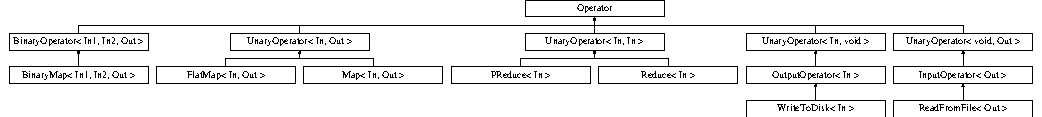
\includegraphics[height=1.568627cm]{class_operator}
\end{center}
\end{figure}
\subsection*{\-Public \-Member \-Functions}
\begin{DoxyCompactItemize}
\item 
virtual std\-::string \hyperlink{class_operator_aabb42a0bffefa195ef28dcb8de28aec1}{name} ()
\item 
\hypertarget{class_operator_ab818c777eba5ea81a1e35bf15cd748ba}{virtual std\-::string {\bfseries name\-\_\-short} ()=0}\label{class_operator_ab818c777eba5ea81a1e35bf15cd748ba}

\end{DoxyCompactItemize}
\subsection*{\-Protected \-Member \-Functions}
\begin{DoxyCompactItemize}
\item 
\hypertarget{class_operator_a6af729a9d00cab0f62cf0e3de2548d39}{virtual bool {\bfseries check\-Input\-Type\-Sanity} (\-Type\-Info\-Ref id)=0}\label{class_operator_a6af729a9d00cab0f62cf0e3de2548d39}

\item 
\hypertarget{class_operator_aeacd17ae40fc541ee6a960ee45e405e6}{virtual bool {\bfseries check\-Output\-Type\-Sanity} (\-Type\-Info\-Ref id)=0}\label{class_operator_aeacd17ae40fc541ee6a960ee45e405e6}

\item 
\hypertarget{class_operator_a5b7ccb315884468f1683e83b3539f400}{virtual const \-Operator\-Class {\bfseries operator\-\_\-class} ()=0}\label{class_operator_a5b7ccb315884468f1683e83b3539f400}

\item 
\hypertarget{class_operator_a7753ef26769c0aa9ab986d51e7d76339}{virtual ff\-::ff\-\_\-node $\ast$ {\bfseries node\-\_\-operator} (size\-\_\-t par\-\_\-deg=1)=0}\label{class_operator_a7753ef26769c0aa9ab986d51e7d76339}

\item 
\hypertarget{class_operator_a2f0f76f195ffd9ee8f1fce2da7956926}{bool $\ast$ {\bfseries structure\-\_\-type} ()}\label{class_operator_a2f0f76f195ffd9ee8f1fce2da7956926}

\item 
\hypertarget{class_operator_a220b5efebda50b93c7fb29d997a12413}{void {\bfseries set\-\_\-input\-\_\-degree} (size\-\_\-t degree)}\label{class_operator_a220b5efebda50b93c7fb29d997a12413}

\item 
\hypertarget{class_operator_a49dbe907baab7d9d5ae44c96074fe873}{size\-\_\-t {\bfseries i\-\_\-degree} () const }\label{class_operator_a49dbe907baab7d9d5ae44c96074fe873}

\item 
\hypertarget{class_operator_a398b346d10ab14d3cb80e5b600219ff9}{void {\bfseries set\-\_\-output\-\_\-degree} (size\-\_\-t degree)}\label{class_operator_a398b346d10ab14d3cb80e5b600219ff9}

\item 
\hypertarget{class_operator_a8f4deb310b1665ae300aa3389d7b58b6}{size\-\_\-t {\bfseries o\-\_\-degree} () const }\label{class_operator_a8f4deb310b1665ae300aa3389d7b58b6}

\item 
\hypertarget{class_operator_aa690c335fa31d9b85f9c2e6271a0b018}{void {\bfseries set\-\_\-stype} (enum \-Raw\-Structure\-Type stype, bool flag)}\label{class_operator_aa690c335fa31d9b85f9c2e6271a0b018}

\item 
\hypertarget{class_operator_a910957044131a074f4fa7be8577a900a}{bool {\bfseries stype} (enum \-Raw\-Structure\-Type stype) const }\label{class_operator_a910957044131a074f4fa7be8577a900a}

\end{DoxyCompactItemize}
\subsection*{\-Friends}
\begin{DoxyCompactItemize}
\item 
\hypertarget{class_operator_adb788d0aa2d64624d3602a985936d7da}{class {\bfseries \-Pipe}}\label{class_operator_adb788d0aa2d64624d3602a985936d7da}

\item 
\hypertarget{class_operator_a54f00cc95ee21e7721a0e74cb07f324e}{class {\bfseries \-Semantic\-D\-A\-G}}\label{class_operator_a54f00cc95ee21e7721a0e74cb07f324e}

\item 
\hypertarget{class_operator_a298bf270ce895db324d65478b3b01f5b}{class {\bfseries \-Par\-Exec\-D\-F}}\label{class_operator_a298bf270ce895db324d65478b3b01f5b}

\item 
\hypertarget{class_operator_aab3ea71fc86db58fd440b9c3c1a739c1}{class {\bfseries \-Sem\-D\-A\-G\-Node}}\label{class_operator_aab3ea71fc86db58fd440b9c3c1a739c1}

\end{DoxyCompactItemize}


\subsection{\-Detailed \-Description}
\-Base class defining a semantic dataflow operator. \-An operator has an input and output cardinality $<$\-I-\/degree, \-O-\/degree$>$, where
\begin{DoxyItemize}
\item \-I-\/degree = 0 if generating input, $>$1 otherwise
\item \-O-\/degree = 0 if collecting output, 1 otherwise
\end{DoxyItemize}

\-Operators have also the specification about the \-Structure \-Type they can manage. 

\subsection{\-Member \-Function \-Documentation}
\hypertarget{class_operator_aabb42a0bffefa195ef28dcb8de28aec1}{\index{\-Operator@{\-Operator}!name@{name}}
\index{name@{name}!Operator@{\-Operator}}
\subsubsection[{name}]{\setlength{\rightskip}{0pt plus 5cm}virtual std\-::string {\bf \-Operator\-::name} (
\begin{DoxyParamCaption}
{}
\end{DoxyParamCaption}
)\hspace{0.3cm}{\ttfamily  \mbox{[}inline, virtual\mbox{]}}}}\label{class_operator_aabb42a0bffefa195ef28dcb8de28aec1}
\-Returns a unique name for the operator. 

\-Reimplemented in \hyperlink{class_write_to_disk_a3b57dac20171d5e166210183bceedea2}{\-Write\-To\-Disk$<$ In $>$}, \hyperlink{class_read_from_file_af509393aad1e80f25fee64991f365bbb}{\-Read\-From\-File$<$ Out $>$}, \hyperlink{class_binary_map_a891da29ca1c109f273e6b0448f261783}{\-Binary\-Map$<$ In1, In2, Out $>$}, and \hyperlink{class_binary_operator_a6df8c4e6dee857f27d870c30d4f65920}{\-Binary\-Operator$<$ In1, In2, Out $>$}.



\-The documentation for this class was generated from the following file\-:\begin{DoxyCompactItemize}
\item 
/home/travis/build/alpha-\/unito/\-Pi\-Co/\-Operators/\-Operator.\-hpp\end{DoxyCompactItemize}

\hypertarget{struct_option_data}{\section{\-Option\-Data \-Struct \-Reference}
\label{struct_option_data}\index{\-Option\-Data@{\-Option\-Data}}
}
\subsection*{\-Public \-Attributes}
\begin{DoxyCompactItemize}
\item 
\hypertarget{struct_option_data_aa251ba05c85ecc3f7a6a2d9e6833167c}{fptype {\bfseries s}}\label{struct_option_data_aa251ba05c85ecc3f7a6a2d9e6833167c}

\item 
\hypertarget{struct_option_data_aa26659a7028a77f5a7a262e56613d49c}{fptype {\bfseries strike}}\label{struct_option_data_aa26659a7028a77f5a7a262e56613d49c}

\item 
\hypertarget{struct_option_data_afd5395299014f314194ebfc9698b0c77}{fptype {\bfseries r}}\label{struct_option_data_afd5395299014f314194ebfc9698b0c77}

\item 
\hypertarget{struct_option_data_afa669f300f15d3a332b260ee111a9058}{fptype {\bfseries divq}}\label{struct_option_data_afa669f300f15d3a332b260ee111a9058}

\item 
\hypertarget{struct_option_data_a4af3d7c170b09e052a19104d167bc446}{fptype {\bfseries v}}\label{struct_option_data_a4af3d7c170b09e052a19104d167bc446}

\item 
\hypertarget{struct_option_data_adabce6a96dac3a882bfa7aff54d68783}{fptype {\bfseries t}}\label{struct_option_data_adabce6a96dac3a882bfa7aff54d68783}

\item 
\hypertarget{struct_option_data_ac699cb4236b49115e979d9e1c381252f}{int {\bfseries \-Option\-Type}}\label{struct_option_data_ac699cb4236b49115e979d9e1c381252f}

\item 
\hypertarget{struct_option_data_a589bc62eabfa5946672400b9f2ad2cba}{fptype {\bfseries divs}}\label{struct_option_data_a589bc62eabfa5946672400b9f2ad2cba}

\item 
\hypertarget{struct_option_data_ade725f66587cd311d2414267aa668310}{fptype {\bfseries \-D\-Grefval}}\label{struct_option_data_ade725f66587cd311d2414267aa668310}

\end{DoxyCompactItemize}


\-The documentation for this struct was generated from the following file\-:\begin{DoxyCompactItemize}
\item 
/home/travis/build/alpha-\/unito/\-Pi\-Co/examples/stock-\/market/black\-\_\-scholes.\-hpp\end{DoxyCompactItemize}

\hypertarget{class_output_operator}{\section{\-Output\-Operator$<$ \-In $>$ \-Class \-Template \-Reference}
\label{class_output_operator}\index{\-Output\-Operator$<$ In $>$@{\-Output\-Operator$<$ In $>$}}
}


{\ttfamily \#include $<$\-Output\-Operator.\-hpp$>$}

\-Inheritance diagram for \-Output\-Operator$<$ \-In $>$\-:\begin{figure}[H]
\begin{center}
\leavevmode
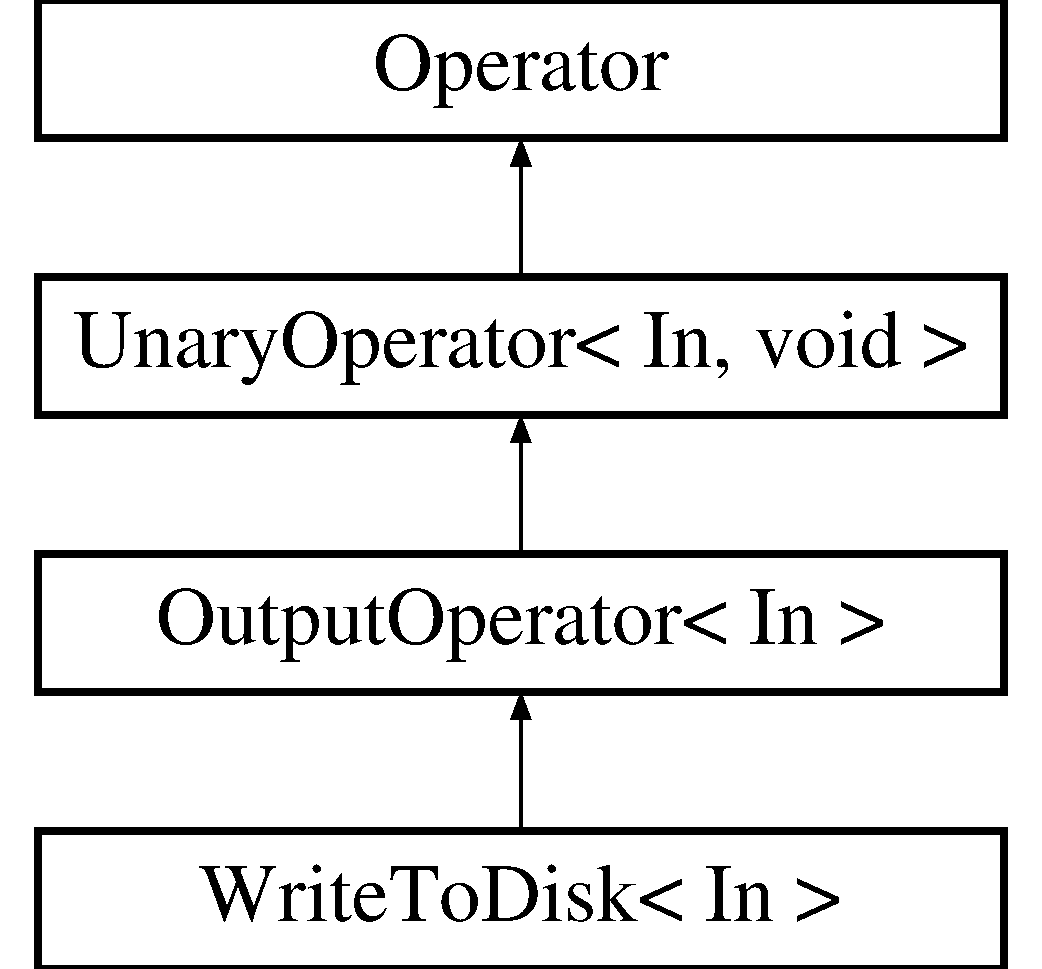
\includegraphics[height=4.000000cm]{class_output_operator}
\end{center}
\end{figure}
\subsection*{\-Public \-Member \-Functions}
\begin{DoxyCompactItemize}
\item 
\hyperlink{class_output_operator_a11cc69b762cccf13c16de81705cb1808}{\-Output\-Operator} (\-Structure\-Type st\-\_\-)
\item 
\hyperlink{class_output_operator_a62379779fb1e0eb3446cb406a8e8d035}{\-Output\-Operator} (const \hyperlink{class_output_operator}{\-Output\-Operator} \&copy)
\item 
std\-::string \hyperlink{class_output_operator_aa0d416361680f33ebd6e1785a97bc3fe}{name\-\_\-short} ()
\item 
\hypertarget{class_output_operator_a71c66a7b3b093947272de215d8706e1f}{virtual void {\bfseries run\-\_\-kernel} (\-In $\ast$)=0}\label{class_output_operator_a71c66a7b3b093947272de215d8706e1f}

\end{DoxyCompactItemize}
\subsection*{\-Protected \-Member \-Functions}
\begin{DoxyCompactItemize}
\item 
\hypertarget{class_output_operator_a76c77bafddc3651ae9afc5ff2a46ba15}{const \-Operator\-Class {\bfseries operator\-\_\-class} ()}\label{class_output_operator_a76c77bafddc3651ae9afc5ff2a46ba15}

\end{DoxyCompactItemize}


\subsection{\-Detailed \-Description}
\subsubsection*{template$<$typename In$>$class Output\-Operator$<$ In $>$}

\-Defines an operator performing the policy for managing output (i.\-e. write on file or standard output). \-It automatically performs a type sanity check on input type.

\-The output kernel is defined by the user and can be a lambda function, a functor or a function.

\-Furthermore, the user specifies the structure of the data type the \hyperlink{class_collector}{\-Collector} generates. \-It can be\-:
\begin{DoxyItemize}
\item \-Bag (spec\-: unordered, bounded)
\item \-List (spec\-: ordered, bounded)
\item \-Stream (spec\-: ordered, unbounded)
\item \-Unbounded \-Bag (spec\-: unordered, unbounded)
\end{DoxyItemize}

\-Its behaviour w.\-r.\-t. composed \-Pipes (with both append and pair) has to be defined. 

\subsection{\-Constructor \& \-Destructor \-Documentation}
\hypertarget{class_output_operator_a11cc69b762cccf13c16de81705cb1808}{\index{\-Output\-Operator@{\-Output\-Operator}!\-Output\-Operator@{\-Output\-Operator}}
\index{\-Output\-Operator@{\-Output\-Operator}!OutputOperator@{\-Output\-Operator}}
\subsubsection[{\-Output\-Operator}]{\setlength{\rightskip}{0pt plus 5cm}template$<$typename In $>$ {\bf \-Output\-Operator}$<$ \-In $>$\-::{\bf \-Output\-Operator} (
\begin{DoxyParamCaption}
\item[{\-Structure\-Type}]{st\-\_\-}
\end{DoxyParamCaption}
)\hspace{0.3cm}{\ttfamily  \mbox{[}inline\mbox{]}}}}\label{class_output_operator_a11cc69b762cccf13c16de81705cb1808}
\-Constructor. \-Creates a new \hyperlink{class_collector}{\-Collector} by defining its kernel function outf\-: \-In -\/$>$ void \hypertarget{class_output_operator_a62379779fb1e0eb3446cb406a8e8d035}{\index{\-Output\-Operator@{\-Output\-Operator}!\-Output\-Operator@{\-Output\-Operator}}
\index{\-Output\-Operator@{\-Output\-Operator}!OutputOperator@{\-Output\-Operator}}
\subsubsection[{\-Output\-Operator}]{\setlength{\rightskip}{0pt plus 5cm}template$<$typename In $>$ {\bf \-Output\-Operator}$<$ \-In $>$\-::{\bf \-Output\-Operator} (
\begin{DoxyParamCaption}
\item[{const {\bf \-Output\-Operator}$<$ \-In $>$ \&}]{copy}
\end{DoxyParamCaption}
)\hspace{0.3cm}{\ttfamily  \mbox{[}inline\mbox{]}}}}\label{class_output_operator_a62379779fb1e0eb3446cb406a8e8d035}
\-Copy constructor 

\subsection{\-Member \-Function \-Documentation}
\hypertarget{class_output_operator_aa0d416361680f33ebd6e1785a97bc3fe}{\index{\-Output\-Operator@{\-Output\-Operator}!name\-\_\-short@{name\-\_\-short}}
\index{name\-\_\-short@{name\-\_\-short}!OutputOperator@{\-Output\-Operator}}
\subsubsection[{name\-\_\-short}]{\setlength{\rightskip}{0pt plus 5cm}template$<$typename In $>$ std\-::string {\bf \-Output\-Operator}$<$ \-In $>$\-::{\bf name\-\_\-short} (
\begin{DoxyParamCaption}
{}
\end{DoxyParamCaption}
)\hspace{0.3cm}{\ttfamily  \mbox{[}inline, virtual\mbox{]}}}}\label{class_output_operator_aa0d416361680f33ebd6e1785a97bc3fe}
\-Returns the name of the operator, consisting in the name of the class. 

\-Implements \hyperlink{class_operator}{\-Operator}.



\-Reimplemented in \hyperlink{class_write_to_disk_ab7f18e8983197d9917d2d045943b00ca}{\-Write\-To\-Disk$<$ In $>$}.



\-The documentation for this class was generated from the following file\-:\begin{DoxyCompactItemize}
\item 
/home/travis/build/alpha-\/unito/\-Pi\-Co/\-Operators/\-In\-Out/\-Output\-Operator.\-hpp\end{DoxyCompactItemize}

\hypertarget{class_par_exec_d_f}{\section{\-Par\-Exec\-D\-F \-Class \-Reference}
\label{class_par_exec_d_f}\index{\-Par\-Exec\-D\-F@{\-Par\-Exec\-D\-F}}
}
\subsection*{\-Public \-Member \-Functions}
\begin{DoxyCompactItemize}
\item 
\hypertarget{class_par_exec_d_f_aef7a4078b19e981b0f6d0654509e2f24}{{\bfseries \-Par\-Exec\-D\-F} (adj\-List $\ast$dag, \hyperlink{class_sem_d_a_g_node}{\-Sem\-D\-A\-G\-Node} $\ast$firstnode\-\_\-, \hyperlink{class_sem_d_a_g_node}{\-Sem\-D\-A\-G\-Node} $\ast$lastnode\-\_\-, \hyperlink{class_operator}{\-Operator} $\ast$firstop\-\_\-, \hyperlink{class_operator}{\-Operator} $\ast$lastop\-\_\-)}\label{class_par_exec_d_f_aef7a4078b19e981b0f6d0654509e2f24}

\item 
\hypertarget{class_par_exec_d_f_a5afb1f6732c4c84461a938b7d13fdf49}{void {\bfseries run} ()}\label{class_par_exec_d_f_a5afb1f6732c4c84461a938b7d13fdf49}

\item 
\hypertarget{class_par_exec_d_f_a57c35909797cac0488ce702d10237b98}{double {\bfseries pipe\-\_\-time} ()}\label{class_par_exec_d_f_a57c35909797cac0488ce702d10237b98}

\end{DoxyCompactItemize}


\-The documentation for this class was generated from the following file\-:\begin{DoxyCompactItemize}
\item 
/home/travis/build/alpha-\/unito/\-Pi\-Co/\-Internals/\-Par\-Exec\-D\-F.\-hpp\end{DoxyCompactItemize}

\hypertarget{class_pipe}{\section{\-Pipe \-Class \-Reference}
\label{class_pipe}\index{\-Pipe@{\-Pipe}}
}


{\ttfamily \#include $<$\-Pipe.\-hpp$>$}

\subsection*{\-Public \-Member \-Functions}
\begin{DoxyCompactItemize}
\item 
\hyperlink{class_pipe_a91ddad07e89d5585b1cf27fa7860e201}{\-Pipe} ()
\item 
{\footnotesize template$<$typename T $>$ }\\\hyperlink{class_pipe_a2112ea3ec975e32d471195d7d37dced9}{\-Pipe} (const \-T \&op)
\item 
{\footnotesize template$<$typename T $>$ }\\\hyperlink{class_pipe_ad634a48b656601f80db6fa413c47b035}{\-Pipe} (const \-T \&\&op)
\item 
{\footnotesize template$<$typename T $>$ }\\\hyperlink{class_pipe}{\-Pipe} \& \hyperlink{class_pipe_aa0577b9eaa033a89b6a76353764eed39}{add} (const \-T \&op)
\item 
{\footnotesize template$<$typename T $>$ }\\\hyperlink{class_pipe}{\-Pipe} \& \hyperlink{class_pipe_af0843b7b6b6c33606fce7a995450678a}{add} (const \-T \&\&op)
\item 
\hyperlink{class_pipe}{\-Pipe} \& \hyperlink{class_pipe_a1772082ed12c8b1df452a40439738138}{to} (const \hyperlink{class_pipe}{\-Pipe} \&pipe)
\item 
{\footnotesize template$<$typename in1 , typename in2 , typename out $>$ }\\\hyperlink{class_pipe}{\-Pipe} \& \hyperlink{class_pipe_a5ddf06055414d4ad0b511596dbf3a390}{pair\-\_\-with} (const \hyperlink{class_binary_operator}{\-Binary\-Operator}$<$ in1, in2, out $>$ \&a, const \hyperlink{class_pipe}{\-Pipe} \&pipe)
\item 
\hyperlink{class_pipe}{\-Pipe} \& \hyperlink{class_pipe_ac07aed5f6efda8248a8d3fe7410df6f2}{merge} (const \hyperlink{class_pipe}{\-Pipe} \&pipe)
\item 
void \hyperlink{class_pipe_a288d5b72778f836c7fbca280bf858976}{print\-\_\-\-D\-A\-G} ()
\item 
void \hyperlink{class_pipe_a6ecb3df1580730102c3e925875962bfd}{run} ()
\item 
void \hyperlink{class_pipe_a305c4d6db780c5e2d46a89f756d9aadf}{to\-\_\-dotfile} (std\-::string filename)
\item 
\hypertarget{class_pipe_a6e0bfcd983a9d63d681e1885c282143a}{void {\bfseries pipe\-\_\-time} ()}\label{class_pipe_a6e0bfcd983a9d63d681e1885c282143a}

\end{DoxyCompactItemize}


\subsection{\-Detailed \-Description}
\-A \hyperlink{class_pipe}{\-Pipe} is a single entity composed by operators. \-It can be created and modified by adding single operators or by appending \-Pipes.

\-Each add or append is done on its right side.

\-A \hyperlink{class_pipe}{\-Pipe} has an input cardinality and an output cardinality $<$\-I-\/degree, \-O-\/degree$>$, where
\begin{DoxyItemize}
\item \-I-\/degree = \{0,1\}
\item \-O-\/degree = \{0,1\}
\end{DoxyItemize}

\-I-\/degree and \-O-\/degree define if the \hyperlink{class_pipe}{\-Pipe} can be executed or not\-: when both are zero, the current \hyperlink{class_pipe}{\-Pipe} has both input and output operators.

\-Each \hyperlink{class_pipe}{\-Pipe} has a \-Structure \-Type specification that identifies the type of data that can be managed.

\-The data type can be\-:
\begin{DoxyItemize}
\item \-Bag (spec\-: unordered, bounded)
\item \-List (spec\-: ordered, bounded)
\item \-Stream (spec\-: ordered, unbounded)
\end{DoxyItemize}

\-A \hyperlink{class_pipe}{\-Pipe} can manage one or more compatible \-Structure \-Types which intersection is not empty. \-The \-Structure \-Type is determined by the \hyperlink{class_emitter}{\-Emitter} since it is coded in the collection, but it can be modified while chaining \-Pipes by computing the intersection of \-Structure \-Types.

\-The following show a simple pseudo-\/code example on how to compose \-Pipes.

\-Pipe\-\_\-\-A -\/-\/-\/-\/-\/-\/-\/-\/-\/-\/-\/-\/-\/-\/-\/-\/-\/-\/-\/-\/-\/-\/-\/-\/-\/-\/-\/-\/-\/-\/-\/-\/-\/-\/-\/-\/-\/-\/-\/ $|$ $|$ $|$ \-Map(f) -\/-\/-\/$>$ \-Map(g) -\/-\/-\/$>$ \-Reduce(h) $|$ $|$ $|$ -\/-\/-\/-\/-\/-\/-\/-\/-\/-\/-\/-\/-\/-\/-\/-\/-\/-\/-\/-\/-\/-\/-\/-\/-\/-\/-\/-\/-\/-\/-\/-\/-\/-\/-\/-\/-\/-\/-\/

$\sim$$\sim$$\sim$$\sim$$\sim$$\sim$$\sim$$\sim$$\sim$$\sim$$\sim$$\sim$$\sim$\{.c\}

\hyperlink{class_pipe}{\-Pipe} \-Pipe\-\_\-\-A(\-Map(f)); \-Pipe\-\_\-\-B(\-Map(g)); \-Pipe\-\_\-\-B.\-add(\-Reduce(h)); \-Pipe\-\_\-\-A.\-to(\-Pipe\-\_\-\-B)); $\sim$$\sim$$\sim$$\sim$$\sim$$\sim$$\sim$$\sim$$\sim$$\sim$$\sim$$\sim$$\sim$

\-This example produces a \hyperlink{class_pipe}{\-Pipe} \-Pipe\-\_\-\-A by appending \-Pipe\-\_\-\-B on its right side. \-The resulting pipe has \-I-\/degree and \-O-\/degree 1. \-This \hyperlink{class_pipe}{\-Pipe} can manage all the \-Structure \-Types specifications.

\-When composing \-Pipes with other \-Pipes or \-Operators (to or add methods), the resulting \-I/\-O cardinality must be at most one. 

\subsection{\-Constructor \& \-Destructor \-Documentation}
\hypertarget{class_pipe_a91ddad07e89d5585b1cf27fa7860e201}{\index{\-Pipe@{\-Pipe}!\-Pipe@{\-Pipe}}
\index{\-Pipe@{\-Pipe}!Pipe@{\-Pipe}}
\subsubsection[{\-Pipe}]{\setlength{\rightskip}{0pt plus 5cm}{\bf \-Pipe\-::\-Pipe} (
\begin{DoxyParamCaption}
{}
\end{DoxyParamCaption}
)\hspace{0.3cm}{\ttfamily  \mbox{[}inline\mbox{]}}}}\label{class_pipe_a91ddad07e89d5585b1cf27fa7860e201}
\-Create an empty \hyperlink{class_pipe}{\-Pipe} \hypertarget{class_pipe_a2112ea3ec975e32d471195d7d37dced9}{\index{\-Pipe@{\-Pipe}!\-Pipe@{\-Pipe}}
\index{\-Pipe@{\-Pipe}!Pipe@{\-Pipe}}
\subsubsection[{\-Pipe}]{\setlength{\rightskip}{0pt plus 5cm}template$<$typename T $>$ {\bf \-Pipe\-::\-Pipe} (
\begin{DoxyParamCaption}
\item[{const \-T \&}]{op}
\end{DoxyParamCaption}
)\hspace{0.3cm}{\ttfamily  \mbox{[}inline\mbox{]}}}}\label{class_pipe_a2112ea3ec975e32d471195d7d37dced9}
\-Create a \hyperlink{class_pipe}{\-Pipe} from an initial operator \hypertarget{class_pipe_ad634a48b656601f80db6fa413c47b035}{\index{\-Pipe@{\-Pipe}!\-Pipe@{\-Pipe}}
\index{\-Pipe@{\-Pipe}!Pipe@{\-Pipe}}
\subsubsection[{\-Pipe}]{\setlength{\rightskip}{0pt plus 5cm}template$<$typename T $>$ {\bf \-Pipe\-::\-Pipe} (
\begin{DoxyParamCaption}
\item[{const \-T \&\&}]{op}
\end{DoxyParamCaption}
)\hspace{0.3cm}{\ttfamily  \mbox{[}inline\mbox{]}}}}\label{class_pipe_ad634a48b656601f80db6fa413c47b035}
\-Create a \hyperlink{class_pipe}{\-Pipe} from an initial operator (move) 

\subsection{\-Member \-Function \-Documentation}
\hypertarget{class_pipe_aa0577b9eaa033a89b6a76353764eed39}{\index{\-Pipe@{\-Pipe}!add@{add}}
\index{add@{add}!Pipe@{\-Pipe}}
\subsubsection[{add}]{\setlength{\rightskip}{0pt plus 5cm}template$<$typename T $>$ {\bf \-Pipe}\& \-Pipe\-::add (
\begin{DoxyParamCaption}
\item[{const \-T \&}]{op}
\end{DoxyParamCaption}
)\hspace{0.3cm}{\ttfamily  \mbox{[}inline\mbox{]}}}}\label{class_pipe_aa0577b9eaa033a89b6a76353764eed39}
\-Add a new stage to the \hyperlink{class_pipe}{\-Pipe}.

\begin{DoxyRefDesc}{\-Todo}
\item[\hyperlink{todo__todo000001}{\-Todo}]op should be const \end{DoxyRefDesc}
\hypertarget{class_pipe_af0843b7b6b6c33606fce7a995450678a}{\index{\-Pipe@{\-Pipe}!add@{add}}
\index{add@{add}!Pipe@{\-Pipe}}
\subsubsection[{add}]{\setlength{\rightskip}{0pt plus 5cm}template$<$typename T $>$ {\bf \-Pipe}\& \-Pipe\-::add (
\begin{DoxyParamCaption}
\item[{const \-T \&\&}]{op}
\end{DoxyParamCaption}
)\hspace{0.3cm}{\ttfamily  \mbox{[}inline\mbox{]}}}}\label{class_pipe_af0843b7b6b6c33606fce7a995450678a}
\-Add a new stage to the \hyperlink{class_pipe}{\-Pipe} (move). \hypertarget{class_pipe_ac07aed5f6efda8248a8d3fe7410df6f2}{\index{\-Pipe@{\-Pipe}!merge@{merge}}
\index{merge@{merge}!Pipe@{\-Pipe}}
\subsubsection[{merge}]{\setlength{\rightskip}{0pt plus 5cm}{\bf \-Pipe}\& {\bf \-Pipe\-::merge} (
\begin{DoxyParamCaption}
\item[{const {\bf \-Pipe} \&}]{pipe}
\end{DoxyParamCaption}
)\hspace{0.3cm}{\ttfamily  \mbox{[}inline\mbox{]}}}}\label{class_pipe_ac07aed5f6efda8248a8d3fe7410df6f2}
\-Merges data coming from the current \hyperlink{class_pipe}{\-Pipe} and the one passed as argument. \-The resulting collection is the union of the collection of the two \-Pipes. \-If the input collections are ordered, the order is respected only within each input collections, while there exists some interleaving of the two collections in the resulting one. \-Merging fails if\-:
\begin{DoxyItemize}
\item the current \-O-\/\-Degree is zero and the \hyperlink{class_pipe}{\-Pipe} is not empty
\item output and input data types of the two \-Pipes are not compatible
\item \-Structure \-Types the two \-Pipes are not compatible
\end{DoxyItemize}


\begin{DoxyParams}{\-Parameters}
{\em pipe} & \hyperlink{class_pipe}{\-Pipe} to merge \\
\hline
\end{DoxyParams}
\hypertarget{class_pipe_a5ddf06055414d4ad0b511596dbf3a390}{\index{\-Pipe@{\-Pipe}!pair\-\_\-with@{pair\-\_\-with}}
\index{pair\-\_\-with@{pair\-\_\-with}!Pipe@{\-Pipe}}
\subsubsection[{pair\-\_\-with}]{\setlength{\rightskip}{0pt plus 5cm}template$<$typename in1 , typename in2 , typename out $>$ {\bf \-Pipe}\& {\bf \-Pipe\-::pair\-\_\-with} (
\begin{DoxyParamCaption}
\item[{const {\bf \-Binary\-Operator}$<$ in1, in2, out $>$ \&}]{a, }
\item[{const {\bf \-Pipe} \&}]{pipe}
\end{DoxyParamCaption}
)\hspace{0.3cm}{\ttfamily  \mbox{[}inline\mbox{]}}}}\label{class_pipe_a5ddf06055414d4ad0b511596dbf3a390}
\-Pair the current \hyperlink{class_pipe}{\-Pipe} with a second pipe by a \hyperlink{class_binary_operator}{\-Binary\-Operator} that combines the two input items (a pair) with the function specified by the user. \-This method fails if\-:
\begin{DoxyItemize}
\item the current \-O-\/degree is zero and the \hyperlink{class_pipe}{\-Pipe} is not empty
\item output and input data types of the \-O-\/\-Degree==1 input are not compatible
\item \-Structure \-Types are not compatible 
\begin{DoxyParams}{\-Parameters}
{\em a} & is a \hyperlink{class_binary_operator}{\-Binary\-Operator} \\
\hline
{\em pipe} & is the second input \hyperlink{class_pipe}{\-Pipe} \\
\hline
\end{DoxyParams}

\end{DoxyItemize}\hypertarget{class_pipe_a288d5b72778f836c7fbca280bf858976}{\index{\-Pipe@{\-Pipe}!print\-\_\-\-D\-A\-G@{print\-\_\-\-D\-A\-G}}
\index{print\-\_\-\-D\-A\-G@{print\-\_\-\-D\-A\-G}!Pipe@{\-Pipe}}
\subsubsection[{print\-\_\-\-D\-A\-G}]{\setlength{\rightskip}{0pt plus 5cm}void {\bf \-Pipe\-::print\-\_\-\-D\-A\-G} (
\begin{DoxyParamCaption}
{}
\end{DoxyParamCaption}
)\hspace{0.3cm}{\ttfamily  \mbox{[}inline\mbox{]}}}}\label{class_pipe_a288d5b72778f836c7fbca280bf858976}
\-Print the \-D\-A\-G in two subsequent format\-:
\begin{DoxyItemize}
\item \-Adjacency list
\item \-B\-F\-S visit 
\end{DoxyItemize}\hypertarget{class_pipe_a6ecb3df1580730102c3e925875962bfd}{\index{\-Pipe@{\-Pipe}!run@{run}}
\index{run@{run}!Pipe@{\-Pipe}}
\subsubsection[{run}]{\setlength{\rightskip}{0pt plus 5cm}void {\bf \-Pipe\-::run} (
\begin{DoxyParamCaption}
{}
\end{DoxyParamCaption}
)\hspace{0.3cm}{\ttfamily  \mbox{[}inline\mbox{]}}}}\label{class_pipe_a6ecb3df1580730102c3e925875962bfd}
\-Executes the \hyperlink{class_pipe}{\-Pipe} \hypertarget{class_pipe_a1772082ed12c8b1df452a40439738138}{\index{\-Pipe@{\-Pipe}!to@{to}}
\index{to@{to}!Pipe@{\-Pipe}}
\subsubsection[{to}]{\setlength{\rightskip}{0pt plus 5cm}{\bf \-Pipe}\& {\bf \-Pipe\-::to} (
\begin{DoxyParamCaption}
\item[{const {\bf \-Pipe} \&}]{pipe}
\end{DoxyParamCaption}
)\hspace{0.3cm}{\ttfamily  \mbox{[}inline\mbox{]}}}}\label{class_pipe_a1772082ed12c8b1df452a40439738138}
\-Append a \hyperlink{class_pipe}{\-Pipe} to the current one. \-Operators in the \hyperlink{class_pipe}{\-Pipe} to append are copied into the current one. \-This method fails if\-:
\begin{DoxyItemize}
\item the current \-O-\/\-Degree is zero and the \hyperlink{class_pipe}{\-Pipe} is not empty
\item output and input data types are not compatible
\item \-Structure \-Types are not compatible 
\begin{DoxyParams}{\-Parameters}
{\em pipe} & \hyperlink{class_pipe}{\-Pipe} to append \\
\hline
\end{DoxyParams}

\end{DoxyItemize}\hypertarget{class_pipe_a305c4d6db780c5e2d46a89f756d9aadf}{\index{\-Pipe@{\-Pipe}!to\-\_\-dotfile@{to\-\_\-dotfile}}
\index{to\-\_\-dotfile@{to\-\_\-dotfile}!Pipe@{\-Pipe}}
\subsubsection[{to\-\_\-dotfile}]{\setlength{\rightskip}{0pt plus 5cm}void {\bf \-Pipe\-::to\-\_\-dotfile} (
\begin{DoxyParamCaption}
\item[{std\-::string}]{filename}
\end{DoxyParamCaption}
)\hspace{0.3cm}{\ttfamily  \mbox{[}inline\mbox{]}}}}\label{class_pipe_a305c4d6db780c5e2d46a89f756d9aadf}
\-Encodes the \-D\-A\-G into a dot file. 
\begin{DoxyParams}{\-Parameters}
{\em filename} & dot file \\
\hline
\end{DoxyParams}


\-The documentation for this class was generated from the following file\-:\begin{DoxyCompactItemize}
\item 
/home/travis/build/alpha-\/unito/\-Pi\-Co/\-Pipe.\-hpp\end{DoxyCompactItemize}

\hypertarget{class_p_reduce}{\section{\-P\-Reduce$<$ \-In $>$ \-Class \-Template \-Reference}
\label{class_p_reduce}\index{\-P\-Reduce$<$ In $>$@{\-P\-Reduce$<$ In $>$}}
}


{\ttfamily \#include $<$\-P\-Reduce.\-hpp$>$}

\-Inheritance diagram for \-P\-Reduce$<$ \-In $>$\-:\begin{figure}[H]
\begin{center}
\leavevmode
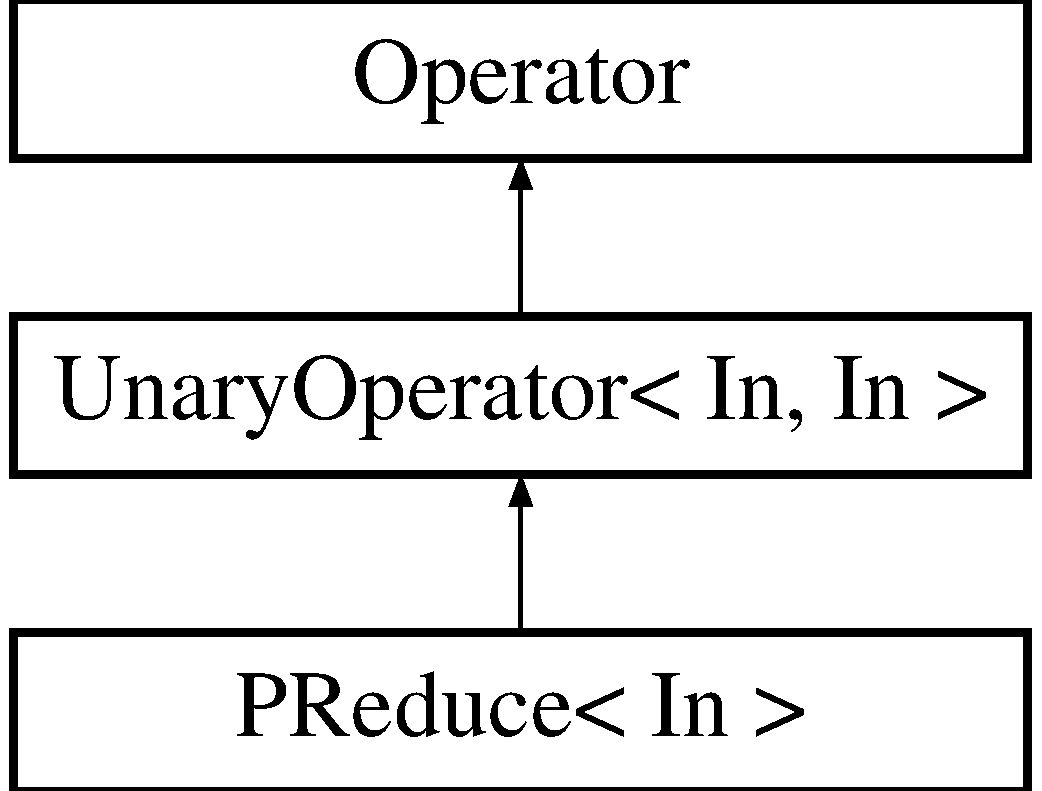
\includegraphics[height=3.000000cm]{class_p_reduce}
\end{center}
\end{figure}
\subsection*{\-Public \-Member \-Functions}
\begin{DoxyCompactItemize}
\item 
\hyperlink{class_p_reduce_a31e0899ba12232bd9d629281a145c219}{\-P\-Reduce} (std\-::function$<$ \-In(\-In, \-In)$>$ reducef\-\_\-)
\item 
std\-::string \hyperlink{class_p_reduce_aeec2fa6ffc97684cc42b6dda26d498d4}{name\-\_\-short} ()
\end{DoxyCompactItemize}
\subsection*{\-Protected \-Member \-Functions}
\begin{DoxyCompactItemize}
\item 
\hypertarget{class_p_reduce_a23d34226d830ba05591373ff0fb745b2}{void {\bfseries run} ()}\label{class_p_reduce_a23d34226d830ba05591373ff0fb745b2}

\item 
\hypertarget{class_p_reduce_af20857bc855fb223be6720efa12f0fb6}{const \-Operator\-Class {\bfseries operator\-\_\-class} ()}\label{class_p_reduce_af20857bc855fb223be6720efa12f0fb6}

\item 
\hypertarget{class_p_reduce_a63a1552b01009c2b13f12f4f25d44603}{ff\-::ff\-\_\-node $\ast$ {\bfseries node\-\_\-operator} (size\-\_\-t par\-\_\-deg)}\label{class_p_reduce_a63a1552b01009c2b13f12f4f25d44603}

\end{DoxyCompactItemize}
\subsection*{\-Friends}
\begin{DoxyCompactItemize}
\item 
\hypertarget{class_p_reduce_adb788d0aa2d64624d3602a985936d7da}{class {\bfseries \-Pipe}}\label{class_p_reduce_adb788d0aa2d64624d3602a985936d7da}

\end{DoxyCompactItemize}


\subsection{\-Detailed \-Description}
\subsubsection*{template$<$typename In$>$class P\-Reduce$<$ In $>$}

\-Defines a \hyperlink{class_p_reduce}{\-P\-Reduce} operator performing a tree reduce function on partitioned input (i.\-e. reduce by key). \-The reduce kernel is defined by the user and can be a lambda function, a functor or a function.

\-The reduce kernel function operates on windows and/or groups if defined on the \hyperlink{class_pipe}{\-Pipe}.

\-It implements a tree reduce operator where input and output value are the same. 

\subsection{\-Constructor \& \-Destructor \-Documentation}
\hypertarget{class_p_reduce_a31e0899ba12232bd9d629281a145c219}{\index{\-P\-Reduce@{\-P\-Reduce}!\-P\-Reduce@{\-P\-Reduce}}
\index{\-P\-Reduce@{\-P\-Reduce}!PReduce@{\-P\-Reduce}}
\subsubsection[{\-P\-Reduce}]{\setlength{\rightskip}{0pt plus 5cm}template$<$typename In $>$ {\bf \-P\-Reduce}$<$ \-In $>$\-::{\bf \-P\-Reduce} (
\begin{DoxyParamCaption}
\item[{std\-::function$<$ \-In(\-In, \-In)$>$}]{reducef\-\_\-}
\end{DoxyParamCaption}
)\hspace{0.3cm}{\ttfamily  \mbox{[}inline\mbox{]}}}}\label{class_p_reduce_a31e0899ba12232bd9d629281a145c219}
\-Constructor. \-Creates a new \hyperlink{class_p_reduce}{\-P\-Reduce} operator by defining its kernel function reducef\-: $<$\-In, \-In$>$ -\/$>$ \-In 

\subsection{\-Member \-Function \-Documentation}
\hypertarget{class_p_reduce_aeec2fa6ffc97684cc42b6dda26d498d4}{\index{\-P\-Reduce@{\-P\-Reduce}!name\-\_\-short@{name\-\_\-short}}
\index{name\-\_\-short@{name\-\_\-short}!PReduce@{\-P\-Reduce}}
\subsubsection[{name\-\_\-short}]{\setlength{\rightskip}{0pt plus 5cm}template$<$typename In $>$ std\-::string {\bf \-P\-Reduce}$<$ \-In $>$\-::{\bf name\-\_\-short} (
\begin{DoxyParamCaption}
{}
\end{DoxyParamCaption}
)\hspace{0.3cm}{\ttfamily  \mbox{[}inline, virtual\mbox{]}}}}\label{class_p_reduce_aeec2fa6ffc97684cc42b6dda26d498d4}
\-Returns the name of the operator, consisting in the name of the class. 

\-Implements \hyperlink{class_operator}{\-Operator}.



\-The documentation for this class was generated from the following file\-:\begin{DoxyCompactItemize}
\item 
/home/travis/build/alpha-\/unito/\-Pi\-Co/\-Operators/\-P\-Reduce.\-hpp\end{DoxyCompactItemize}

\hypertarget{class_p_reduce_f_f_node}{\section{\-P\-Reduce\-F\-F\-Node$<$ \-In $>$ \-Class \-Template \-Reference}
\label{class_p_reduce_f_f_node}\index{\-P\-Reduce\-F\-F\-Node$<$ In $>$@{\-P\-Reduce\-F\-F\-Node$<$ In $>$}}
}
\subsection*{\-Public \-Member \-Functions}
\begin{DoxyCompactItemize}
\item 
\hypertarget{class_p_reduce_f_f_node_a618f505f2a8eb4c8af71229016508356}{{\bfseries \-P\-Reduce\-F\-F\-Node} (std\-::function$<$ \-In(\-In, \-In)$>$ $\ast$preducef)}\label{class_p_reduce_f_f_node_a618f505f2a8eb4c8af71229016508356}

\item 
\hypertarget{class_p_reduce_f_f_node_a6f425a4f78632b76cec0e7658bcf8c3b}{void $\ast$ {\bfseries svc} (void $\ast$task)}\label{class_p_reduce_f_f_node_a6f425a4f78632b76cec0e7658bcf8c3b}

\end{DoxyCompactItemize}
\subsubsection*{template$<$typename \-In$>$ class P\-Reduce\-F\-F\-Node$<$ In $>$}



\-The documentation for this class was generated from the following file\-:\begin{DoxyCompactItemize}
\item 
/home/travis/build/alpha-\/unito/\-Pi\-Co/\-Internals/\-F\-F\-Operators/\-P\-Reduce\-F\-F\-Node.\-hpp\end{DoxyCompactItemize}

\hypertarget{class_read_from_file}{\section{\-Read\-From\-File$<$ \-Out $>$ \-Class \-Template \-Reference}
\label{class_read_from_file}\index{\-Read\-From\-File$<$ Out $>$@{\-Read\-From\-File$<$ Out $>$}}
}


{\ttfamily \#include $<$\-Read\-From\-File.\-hpp$>$}

\-Inheritance diagram for \-Read\-From\-File$<$ \-Out $>$\-:\begin{figure}[H]
\begin{center}
\leavevmode
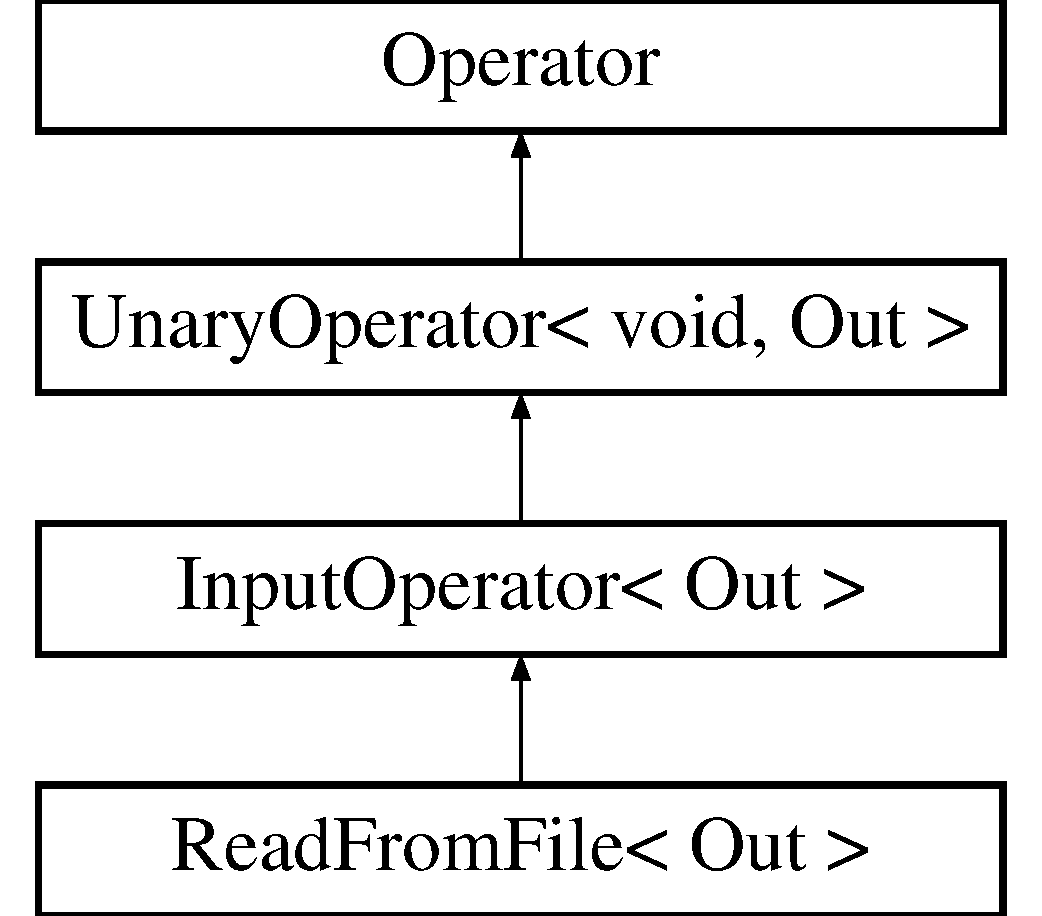
\includegraphics[height=4.000000cm]{class_read_from_file}
\end{center}
\end{figure}
\subsection*{\-Public \-Member \-Functions}
\begin{DoxyCompactItemize}
\item 
\hyperlink{class_read_from_file_abe2865029ef79f9dd35e511892738dc8}{\-Read\-From\-File} (std\-::string filename\-\_\-, std\-::function$<$ \-Out(std\-::string)$>$ func\-\_\-)
\item 
\hyperlink{class_read_from_file_aecb083f7807d61a59bcfe3394d9aa808}{\-Read\-From\-File} (const \hyperlink{class_read_from_file}{\-Read\-From\-File} \&copy)
\item 
std\-::string \hyperlink{class_read_from_file_af509393aad1e80f25fee64991f365bbb}{name} ()
\item 
std\-::string \hyperlink{class_read_from_file_a58ff16dcafb4ad2039cf151fd7a0440f}{name\-\_\-short} ()
\end{DoxyCompactItemize}
\subsection*{\-Protected \-Member \-Functions}
\begin{DoxyCompactItemize}
\item 
\hypertarget{class_read_from_file_af1d716032c6d0b662aba9318584b14ff}{void {\bfseries run\-\_\-kernel} ()}\label{class_read_from_file_af1d716032c6d0b662aba9318584b14ff}

\item 
\hypertarget{class_read_from_file_a1cb0beec0a2db61f86dea66931373726}{const \-Operator\-Class {\bfseries operator\-\_\-class} ()}\label{class_read_from_file_a1cb0beec0a2db61f86dea66931373726}

\item 
\hypertarget{class_read_from_file_a09f10e5b2ab8a1e303dc0e700fe726f0}{ff\-::ff\-\_\-node $\ast$ {\bfseries node\-\_\-operator} (size\-\_\-t parallelism)}\label{class_read_from_file_a09f10e5b2ab8a1e303dc0e700fe726f0}

\end{DoxyCompactItemize}


\subsection{\-Detailed \-Description}
\subsubsection*{template$<$typename Out$>$class Read\-From\-File$<$ Out $>$}

\-Defines an operator that reads data from a text file and produces an \-Ordered+\-Buonded collection (i.\-e. \-L\-I\-S\-T).

\-The user specifies the kernel function that operates on each line of the text file, passed as a std\-::string. \-The kernel can be a lambda function, a functor or a function.

\-The operator is global and unique for the \hyperlink{class_pipe}{\-Pipe} it refers to. 

\subsection{\-Constructor \& \-Destructor \-Documentation}
\hypertarget{class_read_from_file_abe2865029ef79f9dd35e511892738dc8}{\index{\-Read\-From\-File@{\-Read\-From\-File}!\-Read\-From\-File@{\-Read\-From\-File}}
\index{\-Read\-From\-File@{\-Read\-From\-File}!ReadFromFile@{\-Read\-From\-File}}
\subsubsection[{\-Read\-From\-File}]{\setlength{\rightskip}{0pt plus 5cm}template$<$typename Out $>$ {\bf \-Read\-From\-File}$<$ \-Out $>$\-::{\bf \-Read\-From\-File} (
\begin{DoxyParamCaption}
\item[{std\-::string}]{filename\-\_\-, }
\item[{std\-::function$<$ \-Out(std\-::string)$>$}]{func\-\_\-}
\end{DoxyParamCaption}
)\hspace{0.3cm}{\ttfamily  \mbox{[}inline\mbox{]}}}}\label{class_read_from_file_abe2865029ef79f9dd35e511892738dc8}
\-Constructor. \-Creates a new \hyperlink{class_read_from_file}{\-Read\-From\-File} operator by defining its kernel function\-: std\-::string -\/$>$ \-Out operating on each line of the textfile specified. \hypertarget{class_read_from_file_aecb083f7807d61a59bcfe3394d9aa808}{\index{\-Read\-From\-File@{\-Read\-From\-File}!\-Read\-From\-File@{\-Read\-From\-File}}
\index{\-Read\-From\-File@{\-Read\-From\-File}!ReadFromFile@{\-Read\-From\-File}}
\subsubsection[{\-Read\-From\-File}]{\setlength{\rightskip}{0pt plus 5cm}template$<$typename Out $>$ {\bf \-Read\-From\-File}$<$ \-Out $>$\-::{\bf \-Read\-From\-File} (
\begin{DoxyParamCaption}
\item[{const {\bf \-Read\-From\-File}$<$ \-Out $>$ \&}]{copy}
\end{DoxyParamCaption}
)\hspace{0.3cm}{\ttfamily  \mbox{[}inline\mbox{]}}}}\label{class_read_from_file_aecb083f7807d61a59bcfe3394d9aa808}
\-Copy constructor. 

\subsection{\-Member \-Function \-Documentation}
\hypertarget{class_read_from_file_af509393aad1e80f25fee64991f365bbb}{\index{\-Read\-From\-File@{\-Read\-From\-File}!name@{name}}
\index{name@{name}!ReadFromFile@{\-Read\-From\-File}}
\subsubsection[{name}]{\setlength{\rightskip}{0pt plus 5cm}template$<$typename Out $>$ std\-::string {\bf \-Read\-From\-File}$<$ \-Out $>$\-::{\bf name} (
\begin{DoxyParamCaption}
{}
\end{DoxyParamCaption}
)\hspace{0.3cm}{\ttfamily  \mbox{[}inline, virtual\mbox{]}}}}\label{class_read_from_file_af509393aad1e80f25fee64991f365bbb}
\-Returns a unique name for the operator. 

\-Reimplemented from \hyperlink{class_operator_aabb42a0bffefa195ef28dcb8de28aec1}{\-Operator}.

\hypertarget{class_read_from_file_a58ff16dcafb4ad2039cf151fd7a0440f}{\index{\-Read\-From\-File@{\-Read\-From\-File}!name\-\_\-short@{name\-\_\-short}}
\index{name\-\_\-short@{name\-\_\-short}!ReadFromFile@{\-Read\-From\-File}}
\subsubsection[{name\-\_\-short}]{\setlength{\rightskip}{0pt plus 5cm}template$<$typename Out $>$ std\-::string {\bf \-Read\-From\-File}$<$ \-Out $>$\-::{\bf name\-\_\-short} (
\begin{DoxyParamCaption}
{}
\end{DoxyParamCaption}
)\hspace{0.3cm}{\ttfamily  \mbox{[}inline, virtual\mbox{]}}}}\label{class_read_from_file_a58ff16dcafb4ad2039cf151fd7a0440f}
\-Returns the name of the operator, consisting in the name of the class. 

\-Reimplemented from \hyperlink{class_input_operator_a5f752278e586f9c22535bdffdbbe14d2}{\-Input\-Operator$<$ Out $>$}.



\-The documentation for this class was generated from the following file\-:\begin{DoxyCompactItemize}
\item 
/home/travis/build/alpha-\/unito/\-Pi\-Co/\-Operators/\-In\-Out/\-Read\-From\-File.\-hpp\end{DoxyCompactItemize}

\hypertarget{class_read_from_file_f_f_node}{\section{\-Read\-From\-File\-F\-F\-Node$<$ \-Out $>$ \-Class \-Template \-Reference}
\label{class_read_from_file_f_f_node}\index{\-Read\-From\-File\-F\-F\-Node$<$ Out $>$@{\-Read\-From\-File\-F\-F\-Node$<$ Out $>$}}
}
\subsection*{\-Public \-Member \-Functions}
\begin{DoxyCompactItemize}
\item 
\hypertarget{class_read_from_file_f_f_node_abf7a8aa34e88a9ce0e4767d84363156f}{{\bfseries \-Read\-From\-File\-F\-F\-Node} (std\-::function$<$ \-Out(std\-::string)$>$ kernel\-\_\-, std\-::string filename\-\_\-)}\label{class_read_from_file_f_f_node_abf7a8aa34e88a9ce0e4767d84363156f}

\item 
\hypertarget{class_read_from_file_f_f_node_a0fb617afdb7e1313509aa92caa1b9856}{void $\ast$ {\bfseries svc} (void $\ast$in)}\label{class_read_from_file_f_f_node_a0fb617afdb7e1313509aa92caa1b9856}

\end{DoxyCompactItemize}
\subsubsection*{template$<$typename \-Out$>$ class Read\-From\-File\-F\-F\-Node$<$ Out $>$}



\-The documentation for this class was generated from the following file\-:\begin{DoxyCompactItemize}
\item 
/home/travis/build/alpha-\/unito/\-Pi\-Co/\-Internals/\-F\-F\-Operators/\-In\-Out/\-Read\-From\-File\-F\-F\-Node.\-hpp\end{DoxyCompactItemize}

\hypertarget{class_read_from_file_f_f_node_m_b}{\section{\-Read\-From\-File\-F\-F\-Node\-M\-B$<$ \-Out $>$ \-Class \-Template \-Reference}
\label{class_read_from_file_f_f_node_m_b}\index{\-Read\-From\-File\-F\-F\-Node\-M\-B$<$ Out $>$@{\-Read\-From\-File\-F\-F\-Node\-M\-B$<$ Out $>$}}
}
\subsection*{\-Public \-Member \-Functions}
\begin{DoxyCompactItemize}
\item 
\hypertarget{class_read_from_file_f_f_node_m_b_a16b4ed3bd25ff2ede113f868a3ae2f26}{{\bfseries \-Read\-From\-File\-F\-F\-Node\-M\-B} (std\-::function$<$ \-Out(std\-::string)$>$ kernel\-\_\-, std\-::string filename\-\_\-)}\label{class_read_from_file_f_f_node_m_b_a16b4ed3bd25ff2ede113f868a3ae2f26}

\item 
\hypertarget{class_read_from_file_f_f_node_m_b_aebc4fe338d07c777f2a58001f27597e5}{void $\ast$ {\bfseries svc} (void $\ast$in)}\label{class_read_from_file_f_f_node_m_b_aebc4fe338d07c777f2a58001f27597e5}

\end{DoxyCompactItemize}
\subsubsection*{template$<$typename Out$>$ class Read\-From\-File\-F\-F\-Node\-M\-B$<$ Out $>$}



\-The documentation for this class was generated from the following file\-:\begin{DoxyCompactItemize}
\item 
/home/travis/build/alpha-\/unito/\-Pi\-Co/\-Internals/\-F\-F\-Operators/\-In\-Out/\-Read\-From\-File\-F\-F\-Node\-M\-B.\-hpp\end{DoxyCompactItemize}

\hypertarget{class_reduce}{\section{\-Reduce$<$ \-In $>$ \-Class \-Template \-Reference}
\label{class_reduce}\index{\-Reduce$<$ In $>$@{\-Reduce$<$ In $>$}}
}


{\ttfamily \#include $<$\-Reduce.\-hpp$>$}

\-Inheritance diagram for \-Reduce$<$ \-In $>$\-:\begin{figure}[H]
\begin{center}
\leavevmode
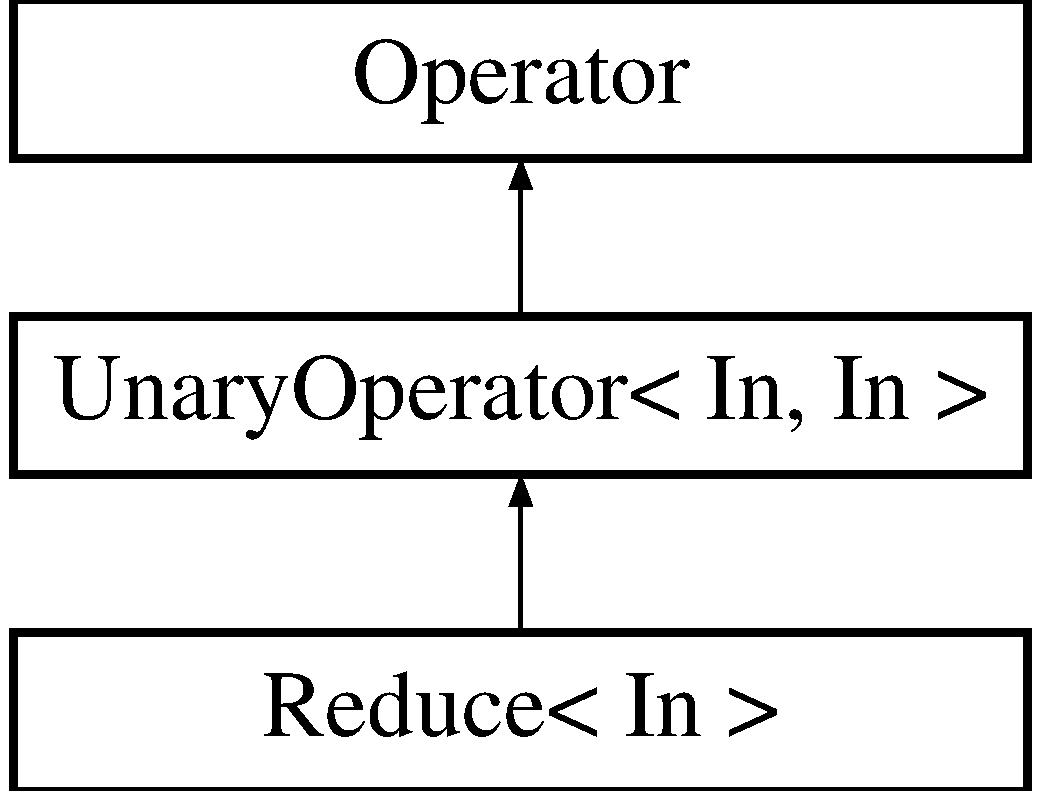
\includegraphics[height=3.000000cm]{class_reduce}
\end{center}
\end{figure}
\subsection*{\-Public \-Member \-Functions}
\begin{DoxyCompactItemize}
\item 
\hyperlink{class_reduce_aca83bb85365a9f7063734f2fe9f98df5}{\-Reduce} (std\-::function$<$ \-In(\-In, \-In)$>$ reducef\-\_\-)
\item 
std\-::string \hyperlink{class_reduce_ac714421091164ce0c8e476f90b6002f0}{name\-\_\-short} ()
\end{DoxyCompactItemize}
\subsection*{\-Protected \-Member \-Functions}
\begin{DoxyCompactItemize}
\item 
\hypertarget{class_reduce_af3e480efa114503bb9bfc2ae363b0750}{void {\bfseries run} ()}\label{class_reduce_af3e480efa114503bb9bfc2ae363b0750}

\item 
\hypertarget{class_reduce_a2b550adc98a8dd58cfe14d51562712b2}{const \-Operator\-Class {\bfseries operator\-\_\-class} ()}\label{class_reduce_a2b550adc98a8dd58cfe14d51562712b2}

\end{DoxyCompactItemize}
\subsection*{\-Friends}
\begin{DoxyCompactItemize}
\item 
\hypertarget{class_reduce_adb788d0aa2d64624d3602a985936d7da}{class {\bfseries \-Pipe}}\label{class_reduce_adb788d0aa2d64624d3602a985936d7da}

\end{DoxyCompactItemize}


\subsection{\-Detailed \-Description}
\subsubsection*{template$<$typename In$>$class Reduce$<$ In $>$}

\-Defines a \hyperlink{class_reduce}{\-Reduce} operator performing a tree reduce function. \-The reduce kernel is defined by the user and can be a lambda function, a functor or a function.

\-The reduce kernel function operates on windows and/or groups if defined on the \hyperlink{class_pipe}{\-Pipe}.

\-It implements a tree reduce operator where input and output value are the same. 

\subsection{\-Constructor \& \-Destructor \-Documentation}
\hypertarget{class_reduce_aca83bb85365a9f7063734f2fe9f98df5}{\index{\-Reduce@{\-Reduce}!\-Reduce@{\-Reduce}}
\index{\-Reduce@{\-Reduce}!Reduce@{\-Reduce}}
\subsubsection[{\-Reduce}]{\setlength{\rightskip}{0pt plus 5cm}template$<$typename In $>$ {\bf \-Reduce}$<$ \-In $>$\-::{\bf \-Reduce} (
\begin{DoxyParamCaption}
\item[{std\-::function$<$ \-In(\-In, \-In)$>$}]{reducef\-\_\-}
\end{DoxyParamCaption}
)\hspace{0.3cm}{\ttfamily  \mbox{[}inline\mbox{]}}}}\label{class_reduce_aca83bb85365a9f7063734f2fe9f98df5}
\-Constructor. \-Creates a new \hyperlink{class_reduce}{\-Reduce} operator by defining its kernel function reducef\-: $<$\-In, \-In$>$ -\/$>$ \-In 

\subsection{\-Member \-Function \-Documentation}
\hypertarget{class_reduce_ac714421091164ce0c8e476f90b6002f0}{\index{\-Reduce@{\-Reduce}!name\-\_\-short@{name\-\_\-short}}
\index{name\-\_\-short@{name\-\_\-short}!Reduce@{\-Reduce}}
\subsubsection[{name\-\_\-short}]{\setlength{\rightskip}{0pt plus 5cm}template$<$typename In $>$ std\-::string {\bf \-Reduce}$<$ \-In $>$\-::{\bf name\-\_\-short} (
\begin{DoxyParamCaption}
{}
\end{DoxyParamCaption}
)\hspace{0.3cm}{\ttfamily  \mbox{[}inline, virtual\mbox{]}}}}\label{class_reduce_ac714421091164ce0c8e476f90b6002f0}
\-Returns the name of the operator, consisting in the name of the class. 

\-Implements \hyperlink{class_operator}{\-Operator}.



\-The documentation for this class was generated from the following file\-:\begin{DoxyCompactItemize}
\item 
/home/travis/build/alpha-\/unito/\-Pi\-Co/\-Operators/\-Reduce.\-hpp\end{DoxyCompactItemize}

\hypertarget{class_r_r_emitter}{\section{\-R\-R\-Emitter \-Class \-Reference}
\label{class_r_r_emitter}\index{\-R\-R\-Emitter@{\-R\-R\-Emitter}}
}
\-Inheritance diagram for \-R\-R\-Emitter\-:\begin{figure}[H]
\begin{center}
\leavevmode
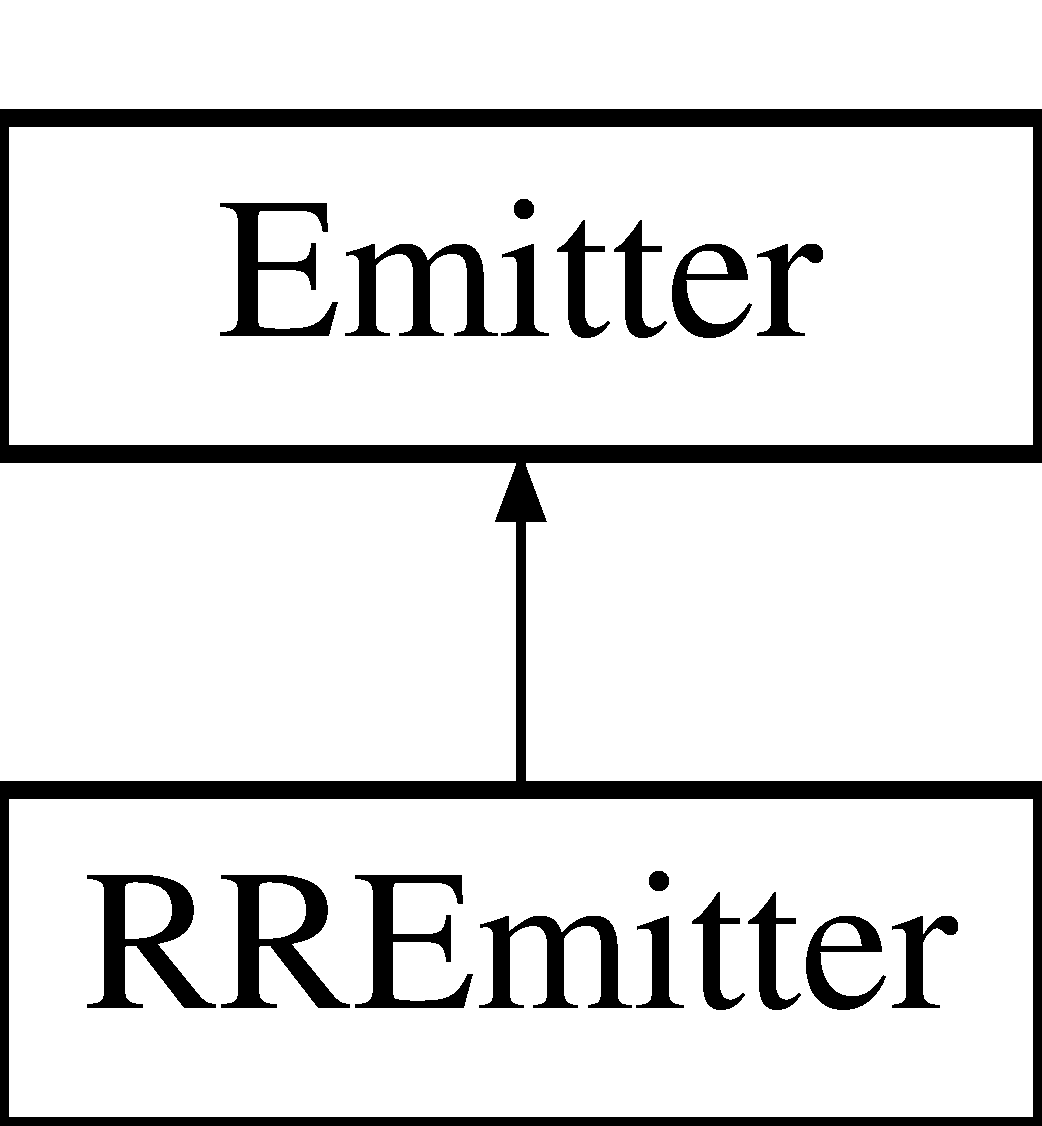
\includegraphics[height=2.000000cm]{class_r_r_emitter}
\end{center}
\end{figure}
\subsection*{\-Public \-Member \-Functions}
\begin{DoxyCompactItemize}
\item 
\hypertarget{class_r_r_emitter_a8c6821b08870a2c8f604d12c7631dd3b}{{\bfseries \-R\-R\-Emitter} (size\-\_\-t nworkers\-\_\-, ff\-\_\-loadbalancer $\ast$const lb\-\_\-)}\label{class_r_r_emitter_a8c6821b08870a2c8f604d12c7631dd3b}

\item 
\hypertarget{class_r_r_emitter_a0d811e077926a3084e9b009b95cf0e16}{int {\bfseries svc\-\_\-init} ()}\label{class_r_r_emitter_a0d811e077926a3084e9b009b95cf0e16}

\item 
\hypertarget{class_r_r_emitter_a388a5d63935e5d1014f75de6ba45003b}{void $\ast$ {\bfseries svc} (void $\ast$task)}\label{class_r_r_emitter_a388a5d63935e5d1014f75de6ba45003b}

\end{DoxyCompactItemize}


\-The documentation for this class was generated from the following file\-:\begin{DoxyCompactItemize}
\item 
/home/travis/build/alpha-\/unito/\-Pi\-Co/\-Internals/\-F\-F\-Operators/\-R\-R\-Emitter.\-hpp\end{DoxyCompactItemize}

\hypertarget{class_semantic_d_a_g}{\section{\-Semantic\-D\-A\-G \-Class \-Reference}
\label{class_semantic_d_a_g}\index{\-Semantic\-D\-A\-G@{\-Semantic\-D\-A\-G}}
}


{\ttfamily \#include $<$\-Semantic\-D\-A\-G.\-hpp$>$}

\subsection*{\-Public \-Member \-Functions}
\begin{DoxyCompactItemize}
\item 
\hypertarget{class_semantic_d_a_g_a63c5a068d3052c88120d5dae11eadb75}{{\bfseries \-Semantic\-D\-A\-G} (std\-::shared\-\_\-ptr$<$ \hyperlink{class_operator}{\-Operator} $>$ start)}\label{class_semantic_d_a_g_a63c5a068d3052c88120d5dae11eadb75}

\item 
\hypertarget{class_semantic_d_a_g_a5af2afb0e5c1c0cd7324c5d9f1e56c07}{bool {\bfseries add\-\_\-operator} (std\-::shared\-\_\-ptr$<$ \hyperlink{class_operator}{\-Operator} $>$ op)}\label{class_semantic_d_a_g_a5af2afb0e5c1c0cd7324c5d9f1e56c07}

\item 
\hypertarget{class_semantic_d_a_g_a30e9c73863637250c511c08e45edfe10}{bool {\bfseries append} (const \hyperlink{class_semantic_d_a_g}{\-Semantic\-D\-A\-G} \&inputg)}\label{class_semantic_d_a_g_a30e9c73863637250c511c08e45edfe10}

\item 
\hypertarget{class_semantic_d_a_g_af6ec0f2552523cb3d246b46a270ae110}{\hyperlink{class_sem_d_a_g_node}{\-Sem\-D\-A\-G\-Node} $\ast$ {\bfseries add\-\_\-bcast\-\_\-block} (std\-::shared\-\_\-ptr$<$ \hyperlink{class_operator}{\-Operator} $>$ merge\-Op)}\label{class_semantic_d_a_g_af6ec0f2552523cb3d246b46a270ae110}

\item 
\hypertarget{class_semantic_d_a_g_af348609410e757f64702206b43e1d645}{void {\bfseries append\-\_\-to} (const \hyperlink{class_semantic_d_a_g}{\-Semantic\-D\-A\-G} \&inputg, \hyperlink{class_sem_d_a_g_node}{\-Sem\-D\-A\-G\-Node} $\ast$\&merge\-Node)}\label{class_semantic_d_a_g_af348609410e757f64702206b43e1d645}

\item 
\hypertarget{class_semantic_d_a_g_aaf2ecd6df14950c2df52a8364acddb1e}{void {\bfseries append\-\_\-merge} (const \hyperlink{class_semantic_d_a_g}{\-Semantic\-D\-A\-G} \&inputg)}\label{class_semantic_d_a_g_aaf2ecd6df14950c2df52a8364acddb1e}

\item 
\hypertarget{class_semantic_d_a_g_a36fea89079fe2cc2b5e3ede3d18fec7f}{void {\bfseries print} ()}\label{class_semantic_d_a_g_a36fea89079fe2cc2b5e3ede3d18fec7f}

\item 
\hypertarget{class_semantic_d_a_g_aeb8e91600df76a367a889359c6d6f153}{void {\bfseries to\-\_\-dotfile} (std\-::string filename)}\label{class_semantic_d_a_g_aeb8e91600df76a367a889359c6d6f153}

\item 
\hypertarget{class_semantic_d_a_g_a09890ba4ecd3b7b7a63bb9877be3c244}{void {\bfseries bfs} ()}\label{class_semantic_d_a_g_a09890ba4ecd3b7b7a63bb9877be3c244}

\item 
\hypertarget{class_semantic_d_a_g_aed8ee7e8480adcec8667a264bcefb58c}{bool {\bfseries empty} ()}\label{class_semantic_d_a_g_aed8ee7e8480adcec8667a264bcefb58c}

\item 
\hypertarget{class_semantic_d_a_g_a9d3369eb56aaea911107704466cf8aec}{\hyperlink{class_sem_d_a_g_node}{\-Sem\-D\-A\-G\-Node} $\ast$ {\bfseries last\-Node} () const }\label{class_semantic_d_a_g_a9d3369eb56aaea911107704466cf8aec}

\item 
\hypertarget{class_semantic_d_a_g_ad3984fc7e22740fbcc3037b2bb2e00cc}{void {\bfseries last\-Node} (\hyperlink{class_sem_d_a_g_node}{\-Sem\-D\-A\-G\-Node} $\ast$node)}\label{class_semantic_d_a_g_ad3984fc7e22740fbcc3037b2bb2e00cc}

\item 
\hypertarget{class_semantic_d_a_g_a9d168ba1bab96cfac9ce2161d9808c7d}{\hyperlink{class_sem_d_a_g_node}{\-Sem\-D\-A\-G\-Node} $\ast$ {\bfseries first\-Node} () const }\label{class_semantic_d_a_g_a9d168ba1bab96cfac9ce2161d9808c7d}

\item 
\hypertarget{class_semantic_d_a_g_a49c425f5f51471dca674bc0856c05f27}{std\-::shared\-\_\-ptr$<$ \hyperlink{class_operator}{\-Operator} $>$ {\bfseries last\-Op} () const }\label{class_semantic_d_a_g_a49c425f5f51471dca674bc0856c05f27}

\item 
\hypertarget{class_semantic_d_a_g_a9c8a61c84df31d1b322f828619d65795}{void {\bfseries last\-Op} (std\-::shared\-\_\-ptr$<$ \hyperlink{class_operator}{\-Operator} $>$ op\-\_\-)}\label{class_semantic_d_a_g_a9c8a61c84df31d1b322f828619d65795}

\item 
\hypertarget{class_semantic_d_a_g_ab96250cbbb40055b878c59e3bdd49961}{std\-::shared\-\_\-ptr$<$ \hyperlink{class_operator}{\-Operator} $>$ {\bfseries first\-Op} () const }\label{class_semantic_d_a_g_ab96250cbbb40055b878c59e3bdd49961}

\item 
\hypertarget{class_semantic_d_a_g_af4c527c88b2d24640e11fa16a8caf6a1}{void {\bfseries run} ()}\label{class_semantic_d_a_g_af4c527c88b2d24640e11fa16a8caf6a1}

\item 
\hypertarget{class_semantic_d_a_g_a08f38d352f8443b9df101dd3d319829e}{size\-\_\-t {\bfseries size} ()}\label{class_semantic_d_a_g_a08f38d352f8443b9df101dd3d319829e}

\item 
\hypertarget{class_semantic_d_a_g_a0c954bbbafef3cbd347b9125a941767f}{double {\bfseries pipe\-\_\-time} ()}\label{class_semantic_d_a_g_a0c954bbbafef3cbd347b9125a941767f}

\end{DoxyCompactItemize}


\subsection{\-Detailed \-Description}
\-The \-Semantic \-D\-A\-G is used to represent the semantics dataflow of the application. \-Vertices represent operators and edges represent data dependencies. \-It is represented with adjacency list implemented by a map. 

\-The documentation for this class was generated from the following file\-:\begin{DoxyCompactItemize}
\item 
/home/travis/build/alpha-\/unito/\-Pi\-Co/\-Internals/\-Graph/\-Semantic\-D\-A\-G.\-hpp\end{DoxyCompactItemize}

\hypertarget{class_sem_d_a_g_node}{\section{\-Sem\-D\-A\-G\-Node \-Class \-Reference}
\label{class_sem_d_a_g_node}\index{\-Sem\-D\-A\-G\-Node@{\-Sem\-D\-A\-G\-Node}}
}
\subsection*{\-Public \-Member \-Functions}
\begin{DoxyCompactItemize}
\item 
\hypertarget{class_sem_d_a_g_node_ada1470e0891b69c0b5ef47375df6f1eb}{{\bfseries \-Sem\-D\-A\-G\-Node} (const \hyperlink{class_sem_d_a_g_node}{\-Sem\-D\-A\-G\-Node} $\ast$node)}\label{class_sem_d_a_g_node_ada1470e0891b69c0b5ef47375df6f1eb}

\item 
\hypertarget{class_sem_d_a_g_node_aa4464f1e30cc1cb1d307abc7b3e04491}{{\bfseries \-Sem\-D\-A\-G\-Node} (std\-::shared\-\_\-ptr$<$ \hyperlink{class_operator}{\-Operator} $>$ op\-\_\-)}\label{class_sem_d_a_g_node_aa4464f1e30cc1cb1d307abc7b3e04491}

\item 
\hypertarget{class_sem_d_a_g_node_aca6ad5fd83da57766e0f0d0dbd303430}{{\bfseries \-Sem\-D\-A\-G\-Node} (\-D\-A\-G\-Node\-Role role\-\_\-, \-Operator\-Class op\-\_\-)}\label{class_sem_d_a_g_node_aca6ad5fd83da57766e0f0d0dbd303430}

\item 
\hypertarget{class_sem_d_a_g_node_aff57e8ea2a78f2d741b902809029cf86}{{\bfseries \-Sem\-D\-A\-G\-Node} (\-D\-A\-G\-Node\-Role role\-\_\-, \-Operator\-Class op\-\_\-, size\-\_\-t farmid\-\_\-)}\label{class_sem_d_a_g_node_aff57e8ea2a78f2d741b902809029cf86}

\item 
\hypertarget{class_sem_d_a_g_node_a378126db24a189d1c5c4e53466044200}{void {\bfseries assign} (std\-::shared\-\_\-ptr$<$ \hyperlink{class_operator}{\-Operator} $>$ op\-\_\-)}\label{class_sem_d_a_g_node_a378126db24a189d1c5c4e53466044200}

\item 
\hypertarget{class_sem_d_a_g_node_a205ba24b858d736d155cf4cc67477bec}{ff\-::ff\-\_\-node $\ast$ {\bfseries node\-\_\-operator} (size\-\_\-t par\-\_\-deg=1)}\label{class_sem_d_a_g_node_a205ba24b858d736d155cf4cc67477bec}

\item 
std\-::string \hyperlink{class_sem_d_a_g_node_a4b4318e6fb92342851d261ffcafc8431}{name} () const 
\item 
\hypertarget{class_sem_d_a_g_node_a2e6ee10ddc285d8de8012ee034b8bca9}{std\-::string {\bfseries name\-\_\-short} () const }\label{class_sem_d_a_g_node_a2e6ee10ddc285d8de8012ee034b8bca9}

\end{DoxyCompactItemize}
\subsection*{\-Public \-Attributes}
\begin{DoxyCompactItemize}
\item 
\hypertarget{class_sem_d_a_g_node_ae7a0d9d27da149bad6e26b89164dce1a}{std\-::shared\-\_\-ptr$<$ \hyperlink{class_operator}{\-Operator} $>$ {\bfseries op}}\label{class_sem_d_a_g_node_ae7a0d9d27da149bad6e26b89164dce1a}

\item 
\hypertarget{class_sem_d_a_g_node_a938dff0f7f403a78d4a9e34dbce7fdb6}{\-D\-A\-G\-Node\-Role {\bfseries role}}\label{class_sem_d_a_g_node_a938dff0f7f403a78d4a9e34dbce7fdb6}

\item 
\hypertarget{class_sem_d_a_g_node_a4a6d752e7bf3c9bb1871c2cfdfb69030}{\-Operator\-Class {\bfseries opclass}}\label{class_sem_d_a_g_node_a4a6d752e7bf3c9bb1871c2cfdfb69030}

\item 
\hypertarget{class_sem_d_a_g_node_a92e650c4fb214ab8e64f30e535dded76}{size\-\_\-t {\bfseries farmid}}\label{class_sem_d_a_g_node_a92e650c4fb214ab8e64f30e535dded76}

\end{DoxyCompactItemize}
\subsection*{\-Static \-Public \-Attributes}
\begin{DoxyCompactItemize}
\item 
\hypertarget{class_sem_d_a_g_node_a796e8c993240ed8d09d9dc36c005557c}{static size\-\_\-t {\bfseries farmidcounter} = 1}\label{class_sem_d_a_g_node_a796e8c993240ed8d09d9dc36c005557c}

\end{DoxyCompactItemize}


\subsection{\-Member \-Function \-Documentation}
\hypertarget{class_sem_d_a_g_node_a4b4318e6fb92342851d261ffcafc8431}{\index{\-Sem\-D\-A\-G\-Node@{\-Sem\-D\-A\-G\-Node}!name@{name}}
\index{name@{name}!SemDAGNode@{\-Sem\-D\-A\-G\-Node}}
\subsubsection[{name}]{\setlength{\rightskip}{0pt plus 5cm}std\-::string {\bf \-Sem\-D\-A\-G\-Node\-::name} (
\begin{DoxyParamCaption}
{}
\end{DoxyParamCaption}
) const\hspace{0.3cm}{\ttfamily  \mbox{[}inline\mbox{]}}}}\label{class_sem_d_a_g_node_a4b4318e6fb92342851d261ffcafc8431}
\-Returns an unique name for the sem\-D\-A\-G\-Node object. 

\-The documentation for this class was generated from the following files\-:\begin{DoxyCompactItemize}
\item 
/home/travis/build/alpha-\/unito/\-Pi\-Co/\-Internals/\-Graph/\-Sem\-D\-A\-G\-Node.\-hpp\item 
/home/travis/build/alpha-\/unito/\-Pi\-Co/\-Internals/\-Graph/\-Semantic\-D\-A\-G.\-hpp\end{DoxyCompactItemize}

\hypertarget{class_unary_flat_map_f_f_node}{\section{\-Unary\-Flat\-Map\-F\-F\-Node$<$ \-In, \-Out $>$ \-Class \-Template \-Reference}
\label{class_unary_flat_map_f_f_node}\index{\-Unary\-Flat\-Map\-F\-F\-Node$<$ In, Out $>$@{\-Unary\-Flat\-Map\-F\-F\-Node$<$ In, Out $>$}}
}
\subsection*{\-Public \-Member \-Functions}
\begin{DoxyCompactItemize}
\item 
\hypertarget{class_unary_flat_map_f_f_node_a499b4632b4942c1e69c889e2d268333b}{{\bfseries \-Unary\-Flat\-Map\-F\-F\-Node} (size\-\_\-t parallelism, std\-::function$<$ std\-::vector$<$ \-Out $>$(\-In)$>$ $\ast$flatmapf)}\label{class_unary_flat_map_f_f_node_a499b4632b4942c1e69c889e2d268333b}

\item 
\hypertarget{class_unary_flat_map_f_f_node_abe8d9f971dd708546ce60daf0fcd3b3f}{void $\ast$ {\bfseries svc} (void $\ast$task)}\label{class_unary_flat_map_f_f_node_abe8d9f971dd708546ce60daf0fcd3b3f}

\end{DoxyCompactItemize}
\subsubsection*{template$<$typename \-In, typename \-Out$>$ class Unary\-Flat\-Map\-F\-F\-Node$<$ In, Out $>$}



\-The documentation for this class was generated from the following file\-:\begin{DoxyCompactItemize}
\item 
/home/travis/build/alpha-\/unito/\-Pi\-Co/\-Internals/\-F\-F\-Operators/\-Unary\-Flat\-Map\-F\-F\-Node.\-hpp\end{DoxyCompactItemize}

\hypertarget{class_unary_map_f_f_node}{\section{\-Unary\-Map\-F\-F\-Node$<$ \-In, \-Out $>$ \-Class \-Template \-Reference}
\label{class_unary_map_f_f_node}\index{\-Unary\-Map\-F\-F\-Node$<$ In, Out $>$@{\-Unary\-Map\-F\-F\-Node$<$ In, Out $>$}}
}
\subsection*{\-Public \-Member \-Functions}
\begin{DoxyCompactItemize}
\item 
\hypertarget{class_unary_map_f_f_node_a858a4d82f74827f951bb3b8c53aeeb3d}{{\bfseries \-Unary\-Map\-F\-F\-Node} (size\-\_\-t parallelism, std\-::function$<$ \-Out(\-In)$>$ $\ast$mapf\-\_\-)}\label{class_unary_map_f_f_node_a858a4d82f74827f951bb3b8c53aeeb3d}

\item 
\hypertarget{class_unary_map_f_f_node_a5c994712fefbef1df5bc44502a8febd8}{void $\ast$ {\bfseries svc} (void $\ast$task)}\label{class_unary_map_f_f_node_a5c994712fefbef1df5bc44502a8febd8}

\end{DoxyCompactItemize}
\subsubsection*{template$<$typename \-In, typename \-Out$>$ class Unary\-Map\-F\-F\-Node$<$ In, Out $>$}



\-The documentation for this class was generated from the following file\-:\begin{DoxyCompactItemize}
\item 
/home/travis/build/alpha-\/unito/\-Pi\-Co/\-Internals/\-F\-F\-Operators/\-Unary\-Map\-F\-F\-Node.\-hpp\end{DoxyCompactItemize}

\hypertarget{class_unary_operator}{\section{\-Unary\-Operator$<$ \-In, \-Out $>$ \-Class \-Template \-Reference}
\label{class_unary_operator}\index{\-Unary\-Operator$<$ In, Out $>$@{\-Unary\-Operator$<$ In, Out $>$}}
}


{\ttfamily \#include $<$\-Unary\-Operator.\-hpp$>$}

\-Inheritance diagram for \-Unary\-Operator$<$ \-In, \-Out $>$\-:\begin{figure}[H]
\begin{center}
\leavevmode
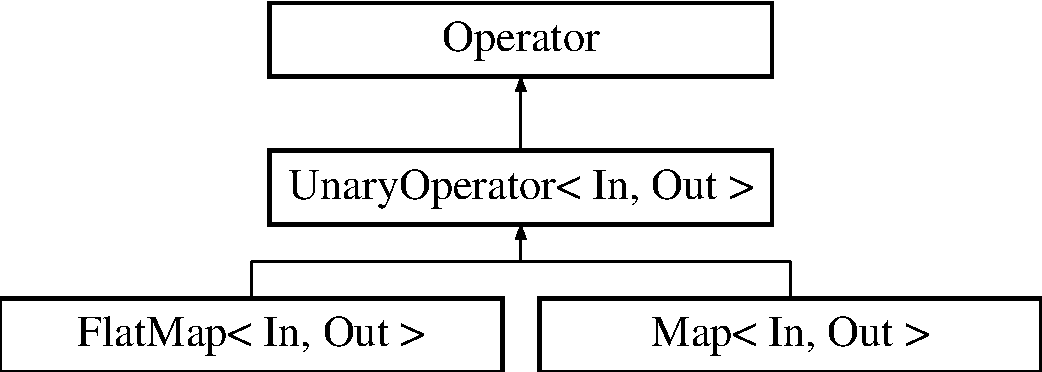
\includegraphics[height=3.000000cm]{class_unary_operator}
\end{center}
\end{figure}
\subsection*{\-Public \-Types}
\begin{DoxyCompactItemize}
\item 
\hypertarget{class_unary_operator_ad5c2571562954f8e0197da4592d23b8d}{typedef \-In {\bfseries in\-T}}\label{class_unary_operator_ad5c2571562954f8e0197da4592d23b8d}

\item 
\hypertarget{class_unary_operator_ad939e9408cfcf42963dbd3c4c314bc4c}{typedef \-Out {\bfseries out\-T}}\label{class_unary_operator_ad939e9408cfcf42963dbd3c4c314bc4c}

\end{DoxyCompactItemize}
\subsection*{\-Public \-Member \-Functions}
\begin{DoxyCompactItemize}
\item 
\hypertarget{class_unary_operator_a3193274926860f4ef1f9d7bd47cfb67e}{{\bfseries \-Unary\-Operator} (const \hyperlink{class_unary_operator}{\-Unary\-Operator} \&copy)}\label{class_unary_operator_a3193274926860f4ef1f9d7bd47cfb67e}

\end{DoxyCompactItemize}
\subsection*{\-Protected \-Member \-Functions}
\begin{DoxyCompactItemize}
\item 
\hypertarget{class_unary_operator_a149286573d17c78732465b5ba66514c2}{virtual bool {\bfseries check\-Input\-Type\-Sanity} (\-Type\-Info\-Ref id)}\label{class_unary_operator_a149286573d17c78732465b5ba66514c2}

\item 
\hypertarget{class_unary_operator_a5dc4cd8d71523d8de26132c8b32aa755}{virtual bool {\bfseries check\-Output\-Type\-Sanity} (\-Type\-Info\-Ref id)}\label{class_unary_operator_a5dc4cd8d71523d8de26132c8b32aa755}

\item 
\hypertarget{class_unary_operator_a2ce8b32a213fb78eacedb2d30f1a1e0e}{virtual const \-Operator\-Class {\bfseries operator\-\_\-class} ()=0}\label{class_unary_operator_a2ce8b32a213fb78eacedb2d30f1a1e0e}

\end{DoxyCompactItemize}
\subsection*{\-Friends}
\begin{DoxyCompactItemize}
\item 
\hypertarget{class_unary_operator_adb788d0aa2d64624d3602a985936d7da}{class {\bfseries \-Pipe}}\label{class_unary_operator_adb788d0aa2d64624d3602a985936d7da}

\end{DoxyCompactItemize}


\subsection{\-Detailed \-Description}
\subsubsection*{template$<$typename \-In, typename \-Out$>$class Unary\-Operator$<$ In, Out $>$}

\-Base class for actor nodes with $\ast$one$\ast$ input stream and $\ast$one$\ast$ output stream, either bound or unbound and grouped or plain. \-It is provided with methods for input/output type checking. 

\-The documentation for this class was generated from the following file\-:\begin{DoxyCompactItemize}
\item 
/home/travis/build/alpha-\/unito/\-Pi\-Co/\-Operators/\-Unary\-Operator.\-hpp\end{DoxyCompactItemize}

\hypertarget{class_window_param}{\section{\-Window\-Param \-Class \-Reference}
\label{class_window_param}\index{\-Window\-Param@{\-Window\-Param}}
}


\-The documentation for this class was generated from the following file\-:\begin{DoxyCompactItemize}
\item 
/home/travis/build/alpha-\/unito/\-Pi\-Co/\-Internals/\-Window\-Param.\-hpp\end{DoxyCompactItemize}

\hypertarget{class_write_to_disk}{\section{\-Write\-To\-Disk$<$ \-In $>$ \-Class \-Template \-Reference}
\label{class_write_to_disk}\index{\-Write\-To\-Disk$<$ In $>$@{\-Write\-To\-Disk$<$ In $>$}}
}


{\ttfamily \#include $<$\-Write\-To\-Disk.\-hpp$>$}

\-Inheritance diagram for \-Write\-To\-Disk$<$ \-In $>$\-:\begin{figure}[H]
\begin{center}
\leavevmode
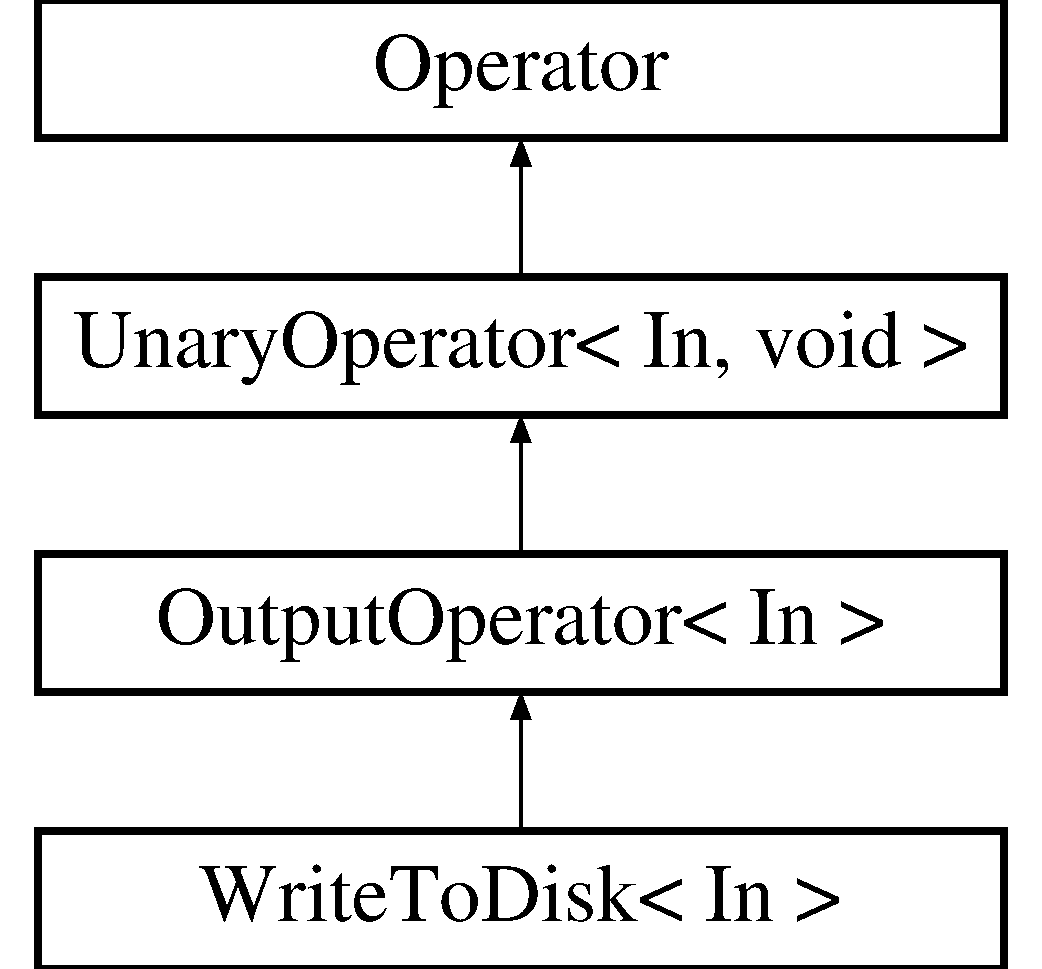
\includegraphics[height=4.000000cm]{class_write_to_disk}
\end{center}
\end{figure}
\subsection*{\-Public \-Member \-Functions}
\begin{DoxyCompactItemize}
\item 
\hyperlink{class_write_to_disk_a32f70bda46bddcfb63fa4dc1c98caaab}{\-Write\-To\-Disk} (std\-::string filename\-\_\-, std\-::function$<$ std\-::string(\-In)$>$ func\-\_\-)
\item 
\hyperlink{class_write_to_disk_abbdea3010854bb53dfef3f5c006fc245}{\-Write\-To\-Disk} (const \hyperlink{class_write_to_disk}{\-Write\-To\-Disk} \&copy)
\item 
std\-::string \hyperlink{class_write_to_disk_a3b57dac20171d5e166210183bceedea2}{name} ()
\item 
std\-::string \hyperlink{class_write_to_disk_ab7f18e8983197d9917d2d045943b00ca}{name\-\_\-short} ()
\end{DoxyCompactItemize}
\subsection*{\-Protected \-Member \-Functions}
\begin{DoxyCompactItemize}
\item 
\hypertarget{class_write_to_disk_a9b5fc69a20e3a5d95d8522711f263104}{void {\bfseries run\-\_\-kernel} (\-In $\ast$task)}\label{class_write_to_disk_a9b5fc69a20e3a5d95d8522711f263104}

\item 
\hyperlink{class_write_to_disk}{\-Write\-To\-Disk}$<$ \-In $>$ $\ast$ \hyperlink{class_write_to_disk_a0f070d389c1624810e727f648e0fc8fd}{clone} ()
\item 
\hypertarget{class_write_to_disk_a5a4d3a2a0018e52510389b7d630ed794}{const \-Operator\-Class {\bfseries operator\-\_\-class} ()}\label{class_write_to_disk_a5a4d3a2a0018e52510389b7d630ed794}

\item 
\hypertarget{class_write_to_disk_a3f1c3d0610a1a08f485c9b7c561de41f}{ff\-::ff\-\_\-node $\ast$ {\bfseries node\-\_\-operator} (int parallelism)}\label{class_write_to_disk_a3f1c3d0610a1a08f485c9b7c561de41f}

\end{DoxyCompactItemize}


\subsection{\-Detailed \-Description}
\subsubsection*{template$<$typename \-In$>$class Write\-To\-Disk$<$ In $>$}

\-Defines an operator that reads data from a text file and produces an \-Ordered+\-Buonded collection (i.\-e. \-L\-I\-S\-T).

\-The user specifies the kernel function that operates on each line of the text file, passed as a std\-::string. \-The kernel can be a lambda function, a functor or a function.

\-The operator is global and unique for the \hyperlink{class_pipe}{\-Pipe} it refers to. 

\subsection{\-Constructor \& \-Destructor \-Documentation}
\hypertarget{class_write_to_disk_a32f70bda46bddcfb63fa4dc1c98caaab}{\index{\-Write\-To\-Disk@{\-Write\-To\-Disk}!\-Write\-To\-Disk@{\-Write\-To\-Disk}}
\index{\-Write\-To\-Disk@{\-Write\-To\-Disk}!WriteToDisk@{\-Write\-To\-Disk}}
\subsubsection[{\-Write\-To\-Disk}]{\setlength{\rightskip}{0pt plus 5cm}template$<$typename \-In$>$ {\bf \-Write\-To\-Disk}$<$ \-In $>$\-::{\bf \-Write\-To\-Disk} (
\begin{DoxyParamCaption}
\item[{std\-::string}]{filename\-\_\-, }
\item[{std\-::function$<$ std\-::string(\-In)$>$}]{func\-\_\-}
\end{DoxyParamCaption}
)\hspace{0.3cm}{\ttfamily  \mbox{[}inline\mbox{]}}}}\label{class_write_to_disk_a32f70bda46bddcfb63fa4dc1c98caaab}
\-Constructor. \-Creates a new \hyperlink{class_write_to_disk}{\-Write\-To\-Disk} operator by defining its kernel function\-: \-In -\/$>$ void writing to the textfile specified. \hypertarget{class_write_to_disk_abbdea3010854bb53dfef3f5c006fc245}{\index{\-Write\-To\-Disk@{\-Write\-To\-Disk}!\-Write\-To\-Disk@{\-Write\-To\-Disk}}
\index{\-Write\-To\-Disk@{\-Write\-To\-Disk}!WriteToDisk@{\-Write\-To\-Disk}}
\subsubsection[{\-Write\-To\-Disk}]{\setlength{\rightskip}{0pt plus 5cm}template$<$typename \-In$>$ {\bf \-Write\-To\-Disk}$<$ \-In $>$\-::{\bf \-Write\-To\-Disk} (
\begin{DoxyParamCaption}
\item[{const {\bf \-Write\-To\-Disk}$<$ \-In $>$ \&}]{copy}
\end{DoxyParamCaption}
)\hspace{0.3cm}{\ttfamily  \mbox{[}inline\mbox{]}}}}\label{class_write_to_disk_abbdea3010854bb53dfef3f5c006fc245}
\-Copy constructor. 

\subsection{\-Member \-Function \-Documentation}
\hypertarget{class_write_to_disk_a0f070d389c1624810e727f648e0fc8fd}{\index{\-Write\-To\-Disk@{\-Write\-To\-Disk}!clone@{clone}}
\index{clone@{clone}!WriteToDisk@{\-Write\-To\-Disk}}
\subsubsection[{clone}]{\setlength{\rightskip}{0pt plus 5cm}template$<$typename \-In$>$ {\bf \-Write\-To\-Disk}$<$\-In$>$$\ast$ {\bf \-Write\-To\-Disk}$<$ \-In $>$\-::{\bf clone} (
\begin{DoxyParamCaption}
{}
\end{DoxyParamCaption}
)\hspace{0.3cm}{\ttfamily  \mbox{[}inline, protected\mbox{]}}}}\label{class_write_to_disk_a0f070d389c1624810e727f648e0fc8fd}
\-Duplicates a \hyperlink{class_write_to_disk}{\-Write\-To\-Disk} with a copy of the kernel function. \begin{DoxyReturn}{\-Returns}
new \hyperlink{class_write_to_disk}{\-Write\-To\-Disk} pointer 
\end{DoxyReturn}
\hypertarget{class_write_to_disk_a3b57dac20171d5e166210183bceedea2}{\index{\-Write\-To\-Disk@{\-Write\-To\-Disk}!name@{name}}
\index{name@{name}!WriteToDisk@{\-Write\-To\-Disk}}
\subsubsection[{name}]{\setlength{\rightskip}{0pt plus 5cm}template$<$typename \-In$>$ std\-::string {\bf \-Write\-To\-Disk}$<$ \-In $>$\-::{\bf name} (
\begin{DoxyParamCaption}
{}
\end{DoxyParamCaption}
)\hspace{0.3cm}{\ttfamily  \mbox{[}inline, virtual\mbox{]}}}}\label{class_write_to_disk_a3b57dac20171d5e166210183bceedea2}
\-Returns a unique name for the operator. 

\-Reimplemented from \hyperlink{class_operator_aabb42a0bffefa195ef28dcb8de28aec1}{\-Operator}.

\hypertarget{class_write_to_disk_ab7f18e8983197d9917d2d045943b00ca}{\index{\-Write\-To\-Disk@{\-Write\-To\-Disk}!name\-\_\-short@{name\-\_\-short}}
\index{name\-\_\-short@{name\-\_\-short}!WriteToDisk@{\-Write\-To\-Disk}}
\subsubsection[{name\-\_\-short}]{\setlength{\rightskip}{0pt plus 5cm}template$<$typename \-In$>$ std\-::string {\bf \-Write\-To\-Disk}$<$ \-In $>$\-::{\bf name\-\_\-short} (
\begin{DoxyParamCaption}
{}
\end{DoxyParamCaption}
)\hspace{0.3cm}{\ttfamily  \mbox{[}inline, virtual\mbox{]}}}}\label{class_write_to_disk_ab7f18e8983197d9917d2d045943b00ca}
\-Returns the name of the operator, consisting in the name of the class. 

\-Reimplemented from \hyperlink{class_output_operator_aa0d416361680f33ebd6e1785a97bc3fe}{\-Output\-Operator$<$ In $>$}.



\-The documentation for this class was generated from the following file\-:\begin{DoxyCompactItemize}
\item 
/home/travis/build/alpha-\/unito/\-Pi\-Co/\-Operators/\-In\-Out/\-Write\-To\-Disk.\-hpp\end{DoxyCompactItemize}

\hypertarget{class_write_to_disk_f_f_node}{\section{\-Write\-To\-Disk\-F\-F\-Node$<$ \-In $>$ \-Class \-Template \-Reference}
\label{class_write_to_disk_f_f_node}\index{\-Write\-To\-Disk\-F\-F\-Node$<$ In $>$@{\-Write\-To\-Disk\-F\-F\-Node$<$ In $>$}}
}
\subsection*{\-Public \-Member \-Functions}
\begin{DoxyCompactItemize}
\item 
\hypertarget{class_write_to_disk_f_f_node_a5b3fa001c7bf954ca01e9e45652f38cf}{{\bfseries \-Write\-To\-Disk\-F\-F\-Node} (std\-::function$<$ std\-::string(\-In)$>$ kernel\-\_\-, std\-::string filename\-\_\-)}\label{class_write_to_disk_f_f_node_a5b3fa001c7bf954ca01e9e45652f38cf}

\item 
\hypertarget{class_write_to_disk_f_f_node_adbb0f820e3e4168e3881e57e6fffb047}{int {\bfseries svc\-\_\-init} ()}\label{class_write_to_disk_f_f_node_adbb0f820e3e4168e3881e57e6fffb047}

\item 
\hypertarget{class_write_to_disk_f_f_node_abfac53a07fd79196f8f84acc05f14122}{void $\ast$ {\bfseries svc} (void $\ast$task)}\label{class_write_to_disk_f_f_node_abfac53a07fd79196f8f84acc05f14122}

\item 
\hypertarget{class_write_to_disk_f_f_node_a6c3c04a03f899fd788ebd5895c1f42cc}{void {\bfseries svc\-\_\-end} ()}\label{class_write_to_disk_f_f_node_a6c3c04a03f899fd788ebd5895c1f42cc}

\end{DoxyCompactItemize}
\subsubsection*{template$<$typename \-In$>$ class Write\-To\-Disk\-F\-F\-Node$<$ In $>$}



\-The documentation for this class was generated from the following file\-:\begin{DoxyCompactItemize}
\item 
/home/travis/build/alpha-\/unito/\-Pi\-Co/\-Internals/\-F\-F\-Operators/\-In\-Out/\-Write\-To\-Disk\-F\-F\-Node.\-hpp\end{DoxyCompactItemize}

\printindex
\end{document}
